This chapter provides an overview of Moltres as a multiphysics
simulation software for molten salt reactors. 
Section \ref{sec:moltres-features}
describes general software features of Moltres, Section
\ref{sec:moltres-physics} expands on the physics models in Moltres, and Section
\ref{sec:moltres-previous} describes previous work to illustrate the current
capabilities in Moltres.

\section{General Features} \label{sec:moltres-features}

This section discusses the general software features of Moltres. The
discussion specifically focuses on robustness, extensibility, and ease of use
as these characteristics represent the hallmarks of a good multiphysics
software \cite{keyes_multiphysics_2013}. These criteria also apply for
assessing \gls{MSR} simulation tools since the nonlinearity of \gls{MSR}
multiphysics analysis and the complexity of advanced reactor designs
necessitate robust, scalable, and flexible computational tools.

Moltres draws many advantages from being developed on MOOSE
\cite{permann_moose_2020}. MOOSE is an open-source, finite-element,
multiphysics framework developed at \gls{INL}. The framework provides a
user-friendly interface for developing multiphysics software through
\gls{OOP} in \texttt{C++} to modularize various
functions relevant to finite-element, multiphysics solvers. In this approach,
MOOSE and MOOSE-based applications break down \glspl{PDE} into individual terms
and store them as individual \texttt{C++ objects} referred to as
\texttt{Kernels}. These \texttt{Kernels} contain functions for calculating
their weak form residual and Jacobian
contributions and other relevant functions required to solve a given
\gls{PDE}. \gls{OOP} in MOOSE simplifies software development
since developers can write new \texttt{Kernels} as child classes in
\texttt{C++} derived from existing \texttt{Kernels} (base classes) which share
similar physics to inherit common functions.
The same philosophy applies for all other systems in MOOSE such as
the \texttt{BCs}, \texttt{Materials}, and \texttt{Postprocessor}
systems for handling relevant boundary conditions, material properties, and
postprocessing calculations, respectively. Overall, this approach also saves
researchers time and effort as they are unencumbered by the technical details
and complexities involved in programming efficient computational tools for
numerical analysis.

\begin{figure}[htb!]
	\centering
	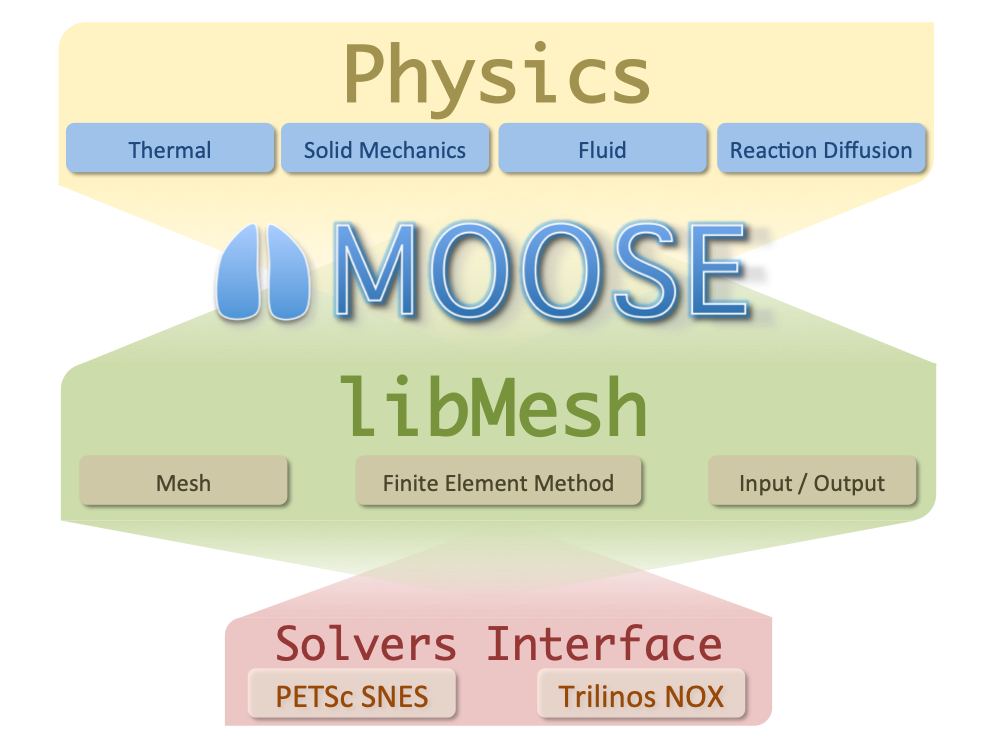
\includegraphics[width=.7\columnwidth]{moose}
	\caption{Structure of MOOSE and its dependencies.}
	\label{fig:moose}
\end{figure}

MOOSE relies on two other open-source libraries: libMesh
\cite{kirk_libmesh_2006} for its \gls{FEM} capabilities on unstructured mesh,
and PETSc \cite{satish_petsc_2019} for its non-linear solvers and
preconditioning routines. By extension, Moltres gains access to these
sophiscated numerical analysis tools and benefits from their continuous
development. Figure
\ref{fig:moose} shows how MOOSE serves as an interface between physics
applications and libMesh/PETSc. MOOSE supports
modeling on up to three-dimensional (3-D) unstructured meshes for a wide range
of mesh file formats, including the commonly used Exodus II file format. For
2-D meshes, users can opt between Cartesian and polar RZ coordinates. MOOSE
also supports parallel computing through the \gls{MPI} library to leverage
modern high-performance computing for large multiphysics simulations.

Moltres benefits from the highly-integrated cross compatibility within the
ecosystem of MOOSE-based applications. MOOSE facilitates multiphysics coupling
among all MOOSE-based applications by providing a common framework for shared
data access and file input/output, thus eliminating computational costs from
data transfers and allowing for fully coupled solves. For example, Moltres
couples with the \texttt{Navier-Stokes} module \cite{peterson_overview_2018}
from MOOSE for fully coupled reactor simulations modeling neutronics and
thermal-hydraulics with incompressible flow. Section
\ref{sec:msr-multiphysics} highlighted the advantages of using fully coupled schemes
for modeling strongly coupled systems such as the coupled
neutronics and thermal-hydraulics in \glspl{MSR}. Moltres can also
couple to other MOOSE-based applications in a similar fashion with ease. In
addition, MOOSE
provides the option for either tight or loose coupling through the
\texttt{MultiApp} system \cite{gaston_physics-based_2015}. Tight coupling
schemes can outperform fully coupled schemes in weakly coupled systems in which
the computational expenses of fully coupled schemes outweigh the savings from
running fewer Newton iterations due to the superior convergence rate. Loose
coupling schemes are useful for accelerating time-dependent simulations of
stable systems towards steady state in which only the steady-state
configuration is of interest to the user. This typically occurs in the later
stages of \gls{MSR} simulations when the delayed neutron precursor
concentrations converge slowly due to their relatively large decay half-lives.
Furthermore, segregated solves through the \texttt{MultiApp} system enables
Moltres to introduce delayed neutron precursor drift and non-uniform
temperature distributions into criticality search simulations. Regardless of
which coupling scheme is best, MOOSE-based applications provide the flexibility
to switch among the schemes as users see fit. For time-dependent simulations,
MOOSE provides more than ten different implicit and explicit timestepping
schemes. The default, most common scheme is the first-order backward Euler
method which offers excellent solver stability for stiff \glspl{PDE}.

Lastly, Moltres is an open-source \gls{LGPL} software hosted on
GitHub \cite{github_build_2017}. Open-sourcing software provides ease of access
and expands the userbase. These characteristics promote software quality
through increased feedback on users' needs and transparency for peer review.
Open-source software accelerate research progress by supporting research
collaboration and sharing best software practices. Supporting Moltres'
continued development, Moltres relies on GitHub for online version control with
continuous integrated testing to protect its existing capabilities.

In summary, Moltres provides robust and flexible coupling capabilities to
model strongly coupled neutronics and thermal-hydraulics in \glspl{MSR}. As a
MOOSE-based application, Moltres is highly extensible by means of coupling to
other MOOSE-based applications and benefits from MOOSE's user-friendly
interface for software development and general ease of use.

\section{Physics Models} \label{sec:moltres-physics}

This section describes the various physics models available in Moltres to model
coupled neutronics and thermal-hydraulics in \glspl{MSR}. Section \ref{sec:nts}
discusses the neutronics model in Moltres, while Section \ref{sec:th} discusses
the thermal-hydraulics model.

\subsection{Neutronics Model} \label{sec:nts}

\subsubsection{Multigroup Neutron Diffusion Model}

Moltres solves the multigroup neutron diffusion equations for the neutron
flux solution within the problem domain. These equations are derived from the
neutron transport equation in the diffusion-dominated limit with Fick's law of
diffusion and further simplified by discretizing the continuous neutron energy
variable into a finite number of energy groups \cite{bell_nuclear_1970,
duderstadt_nuclear_1976}. The time-dependent multigroup neutron
diffusion equations with $G$ energy groups and $I$ delayed neutron precursor
groups are given by:
%
\begin{align}
    \frac{1}{v_g} \frac{\partial \phi_g}{\partial t} =& \nabla \cdot D_g
    \nabla \phi_g - \Sigma^r_g \phi_g +
    \sum^G_{g' \neq g} \Sigma^s_{g' \rightarrow g} \phi_{g'} \nonumber \\
    &+ \chi^p_g \sum^G_{g'=1} \left( 1-\beta \right) \nu \Sigma^f_{g'}
    \phi_{g'} + \chi^d_g \sum^I_i \lambda_i C_i \label{eq:neutron} %\\
%    %
%    \shortintertext{where}
%    v_g =& \text{ average speed of neutrons in group $g$,} 
%    \nonumber \\
%    \phi_g =& \text{ neutron flux in group $g$,}
%    \nonumber \\
%    t =& \text{ time,} \nonumber \\
%    D_g =& \text{ diffusion coefficient of neutrons in group $g$,} \nonumber \\
%    \Sigma^r_g =& \text{ macroscopic removal cross section for} \nonumber \\
%    &\text{ neutrons from group $g$,} \nonumber \\
%    \Sigma^s_{g' \rightarrow g} =& \text{ macroscopic scattering cross section
%    for neutrons from} \nonumber \\
%    &\text{ groups $g'$ to $g$,} \nonumber \\
%    \chi^p_g =& \text{ prompt fission spectrum for neutrons in group $g$,} \nonumber \\
%    G =& \text{ total number of discrete neutron groups,} \nonumber \\
%    \nu_g =& \text{ average number of neutrons produced per fission,} \nonumber
%    \\
%    \Sigma^f_{g} =& \text{ macroscopic fission cross section for neutron}
%    \nonumber \\
%    &\text{ in group $g$,} \nonumber \\
%    \chi^d_g =& \text{ delayed fission spectrum for neutrons in group $g$,} \nonumber \\
%    I =& \text{ total number of delayed neutron precursor groups,} \nonumber \\
%    \beta =& \text{ total delayed neutron fraction.} \nonumber
\end{align}

In spite of forming only around 0.7\% of all neutrons emitted, delayed neutrons
play outsized roles in reactor kinetics. The relatively long half-lives of
delayed neutron precursors gives us ample time in adequately designed reactors
to control reactor power output and intervene in case of power excursions.
The precursor concentration balance equations for $I$ precursor
groups are given by:
%
\begin{align}
    \frac{\partial C_i}{\partial t} =& \beta_i \sum^G_{g'=1} \nu \Sigma^f_{g'}
    \phi_{g'} - \lambda_i C_i - \vec{u} \cdot \nabla C_i + \nabla \cdot
    D_{\text{P}} \nabla C_i \label{eq:precursor} %\\
    %
%    \shortintertext{where}
%    \beta_i =& \text{ delayed neutron fraction of precursor group $i$,}
%    \nonumber \\
%    \lambda_i =& \text{ average decay constant of delayed neutron} \nonumber \\
%    &\text{ precursors in precursor group $i$,} \nonumber \\
%    C_i =& \text{ concentration of delayed neutron precursors in}
%    \nonumber \\
%    &\text{ precursor group $i$,} \nonumber \\
%    \vec{u} =& \text{ molten salt flow velocity vector,}
%    \nonumber \\
%    D_{\text{P}} =& \text{ effective diffusion coefficient of the delayed}
%    \nonumber \\
%    &\text{ neutron precursors.} \nonumber
\end{align}

These two equations are largely similar to conventional formulations of the
multigroup neutron diffusion equations with delayed neutrons for most reactor
types. The only differences are in the last two terms in Equation
\ref{eq:precursor}
which represent the advection and diffusion terms, respectively, to model the
movement of \gls{DNP} in liquid-fuel \glspl{MSR}.

As shown in Equations \ref{eq:neutron} and \ref{eq:precursor}, Moltres requires
group constant data from dedicated high-fidelity neutronics software such as
the NEWT module in SCALE \cite{dehart_reactor_2011}, Serpent
\cite{leppanen_serpent_2014}, or OpenMC \cite{romano_openmc:_2015}. These group
constant data are the neutron energy group $g$ values for $v_g$, $D_g$,
$\Sigma^r_g$, $\Sigma^s_{g' \rightarrow g}$, $\chi^p_g$, $\chi^d_g$,
$\Sigma^f_{g}$, and $\nu\Sigma^f_{g}$, and precursor group $i$ values for
$\beta_i$ and $\lambda_i$. Users
can run a Python script in Moltres' Github repository which automatically reads
user-provided SCALE/Serpent/OpenMC output data files and creates
Moltres-compatible JSON format files containing all required group constant
data. Moltres allows for an arbitrary number of neutron energy groups $G$ and
precursor groups $I$ as long as the user provides the necessary group constant
data. In practice, $I$ depends on the nuclear data library used to generate
group constants---the JEFF \cite{plompen_joint_2020} and ENDF
\cite{brown_endfb-viii0_2018} data libraries define eight precursor groups
and six precursor groups, respectively.

In multiphysics reactor simulations, we model the coupling between neutronics
and thermodynamics through temperature-dependent group constants. To sample
group constants at different temperatures in Moltres, users must provide group
constant data measured at more than one temperature (e.g. 800K--1500K at 100K
intervals). Users can then choose from linear spline, cubic spline, or monotone
cubic interpolation methods available in Moltres to interpolate the group
constant data for values falling within the provided temperature range. 

\subsubsection{Neutronics Model Boundary Conditions}

Moltres provides two types of boundary conditions for neutron fluxes; these are
conventionally known as the vacuum and reflective boundary conditions given,
respectively, as:

\begin{align}
  D_g \nabla \phi_g \cdot \hat{n} + \frac{\phi}{2} =& 0 \label{eq:vacuum}
    \shortintertext{and}
  \nabla \phi \cdot \hat{n} =& 0
    \shortintertext{where}
  \hat{n} =& \mbox{ outward unit normal vector to the boundary.} \nonumber
\end{align}

The vacuum boundary condition typically applies to the external boundaries of
the reactor beyond which lies low-interaction media such as air, while the
reflective boundary condition is useful for exploiting symmetries in the
model geometry such as along the axial boundary in axisymmetric geometries. The
reflective boundary condition is also equivalent to the more generally known
homogeneous Neumann boundary condition. Relevant boundary conditions for
delayed neutron precursors include the homogeneous Neumann boundary condition
along fuel salt-structural interfaces; and outflow/inflow boundary
conditions along the outlet/inlet boundaries through which the precursors
flow as they circulate the fuel salt loop.

\subsection{Thermal-Hydraulics Model} \label{sec:th}

\subsubsection{Incompressible Flow Model}

Moltres largely relies on MOOSE's \texttt{Heat} \texttt{Conduction} and
\texttt{Navier-Stokes} physics modules for its thermal-hydraulics modeling
capabilities. While the \texttt{Navier-Stokes} module supports both
compressible and incompressible flow modeling, this work focuses on
multiphysics coupling in \glspl{MSR} with incompressible flow. The
time-dependent incompressible Navier-Stokes equations for velocity $\vec{u}$
with the Boussinesq approximation for buoyancy-driven flow are given as:

\begin{align}
    \text{Momentum equation: } \rho \frac{\partial \vec{u}}{\partial t} =&
    -\rho (\vec{u}
    \cdot \nabla) \vec{u} - \nabla p + \mu \nabla^2 \vec{u}
    + \rho \alpha \vec{g} \left(T - T_{\text{ref}} \right)
    \label{eq:momemtum}
    \shortintertext{and}
    \text{Mass equation: } \nabla \cdot \vec{u} =& 0
    \label{eq:divergence}
%    \shortintertext{where}
%    \rho =& \text{ fluid density,} \nonumber \\
%    p =& \text{ pressure,} \nonumber \\
%    \mu =& \text{ dynamic viscosity,} \nonumber \\
%    \alpha =& \text{ coefficient of thermal expansion,} \nonumber \\
%    \vec{g} =& \text{ gravitational force vector,} \nonumber
%    \\
%    T =& \text{ fluid temperature,} \nonumber \\
%    T_{\text{ref}} =& \text{ reference temperature at which the nominal}
%    \nonumber \\
%    &\text{ density is provided.} \nonumber
%    \nonumber
\end{align}

Velocity variables and advected quantities such as temperature are susceptible
to numerical node-to-node oscillations
commonly observed when resolving advection-dominated flows using continuous
Galerkin methods \cite{kuhlmann_lid-driven_2018}. The \texttt{Navier-Stokes}
module provides the \gls{SUPG} stabilization scheme
\cite{brooks_streamline_1982} for the velocity and temperature variables to
minimize these oscillations. The module also provides the \gls{PSPG}
stabilization scheme \cite{hughes_new_1986} which enables equal-order
discretizations of pressure and velocity. Peterson et al. \cite{peterson_overview_2018}
provides further detail on the implementation of these stabilization schemes in
the \texttt{Navier-Stokes} module.

\subsubsection{Temperature Advection-Diffusion Model}

Lastly, Moltres solves for the temperature distribution through the temperature
advection-diffusion equation given by:

\begin{align}
    \rho c_{p} \frac{\partial T}{\partial t} =& - \rho c_p \vec{u}
    \cdot \nabla T + \nabla \cdot \left(k \nabla T \right) + Q_f - Q_s
    \label{eq:temp}
    \shortintertext{and}
    Q_f =& \sum^G_{g=1} \epsilon_g \Sigma_g^f \phi_g \label{eq:heat-source}
%    \shortintertext{where}
%    c_p =& \text{ specific heat capacity of molten salt,} \nonumber \\
%    k =& \text{ effective thermal conductivity of molten salt,} \nonumber \\
%    Q_f =& \text{ fission heat source,} \nonumber \\
%    \epsilon_g =& \text{ average fission energy released by neutrons in group
%    $g$,} \nonumber \\
    Q_s =& \text{ heat sink/removal.} \nonumber
\end{align}

$Q_f$ represents the fission heat source term and is calculated by taking the
sum of neutron group fluxes multiplied by their respective macroscopic fission
cross sections and the average fission energy released per fission.

\subsubsection{Thermal-Hydraulics Model Boundary Conditions}

The \texttt{Navier-Stokes} module provides the following types of boundary
conditions for the velocity and temperature variables:

\begin{align}
    \text{Dirichlet: }& & u \ \left(\text{or } T\right) =& c & \\
    \text{Homogeneous Neumann: }& & \frac{\partial u}{\partial x_i} \
    \left(\text{or } \frac{\partial T}{\partial x_i}\right) =& 0 & \\
    \text{``No boundary condition'' outflow: }& &
    \mu \left[ \nabla \vec{u} + \left(\nabla \vec{u} \right)^T \right] \cdot
    \hat{n} =& 0 \ \text{ (velocity)} & \\
    \text{``No boundary condition'' outflow: }& &
    k \nabla T \cdot\hat{n} =& 0 \ \text{ (temperature)} &
    \shortintertext{where}
    & & c =& \text{ user-defined constant value,} & \nonumber \\
    & & \hat{n} =& \text{ unit normal vector to the boundary.} & \nonumber
\end{align}

The Dirichlet boundary condition can be used to set the inlet velocities and
temperatures, and no-slip conditions along solid boundaries, while the
homogeneous Neumann boundary condition is commonly
imposed along the outlet boundary. However, the latter approach tends to
artificially influence upstream behavior, especially in developing flow. The
``no boundary condition'' outflow boundary condition by Griffiths
\cite{griffiths_no_1997} has been shown to reduce such upstream errors.

\subsection{External Loop Model} \label{sec:moltres-loop}

Moltres also accounts for the decay of
\glspl{DNP} outside the active core region by simulating its flow in a
separate 1-D pipe geometry. This outer loop pipe calculation is tightly
coupled to the active core simulation through Picard iterations in MOOSE's
MultiApp functionality and inlet/outlet boundary values.
The outer loop region is assumed to be subcritical to minimize neutron
irradiation upon heat exchangers, pumps, and other equipment. Therefore, the
only significant neutronics-related phenomena are the drift and decay of
\glspl{DNP}. The governing equation for the \glspl{DNP} is:
%
\begin{align}
    \frac{\partial C_i}{\partial t} =& - \lambda_i C_i - u
    \frac{\partial C_i}{\partial x}.
    \label{eq:dnploop}
\end{align}
%
Equation \ref{eq:dnploop} is derived from equation \ref{eq:precursor} by
removing the fission \gls{DNP} source and diffusion terms, and reducing the
dimensionality from 3-D to 1-D.

Moltres also simulates the temperature distribution in the external loop to model heat removal via
heat exchangers. The governing equation
for temperature, derived from equation \ref{eq:temp}, is:
%
\begin{align}
    \rho c_{p} \frac{\partial T}{\partial t} =& - \rho c_p u
    \frac{\partial T}{\partial x} - Q_{hx} \label{eq:temploop}
    \shortintertext{where}
    Q_{hx} =& \text{heat removal rate through the heat exchanger.} 
    \nonumber
\end{align}
%
The fission heat source term is replaced with a heat
exchanger sink term $Q_{hx}$.

\subsubsection{External Loop Model Boundary Conditions}

Table \ref{table:loopbc} lists the boundary conditions for all variables on the inlet and outlet of
the 1-D outer loop region. The inlet boundary conditions are all Dirichlet boundary conditions. The
prescribed value for the inlet boundary conditions are set to match the average outflow from the
active core region. The outlet boundary conditions are all outflow boundary conditions as shown in
Table \ref{table:loopbc}.

\begin{table}[htbp!]
    \small
	\caption{Boundary conditions in the 1-D outer loop geometry. $u$
	represents the 1-D velocity in this region.}
	\centering
	\begin{tabular}{ l l c}
		\toprule
		Variable & Boundary & Boundary Condition \\
        \midrule
        \multirow{2}{*}{Delayed neutron precursor concentration $C_i$} &
        Inlet (Core) & $C_i = c$ \\
        & Outlet (Core) & $u \cdot C_i = 0$ \\
        \midrule
        \multirow{2}{*}{Temperature $T$} &
        Inlet (Core) & $T = c$ \\
        & Outlet (Core) & $u \cdot T = 0$ \\
		\bottomrule
	\end{tabular}
	\label{table:loopbc}
\end{table}

\subsubsection{Core and Outer Loop Coupling Model}

This subsection details the delayed neutron precursors, and
temperature coupling between the core and outer loop regions. 

At every timestep, Moltres calculates weighted averages of the
temperature and the precursors at the outlet. These values are weighted by the
outflow velocity values at the outlet according to the following equation:
%
\begin{align}
    \overline{\psi} =& \frac{\int_\mathcal{C} Y(x_j) u(x_j) dx_j}{
    \int_\mathcal{C} u(x_j) dx_j} \\
    \shortintertext{where}
    Y =& \text{ variable to be weighted} \nonumber \\
    \mathcal{C} =& \text{ outlet boundary area} \nonumber \\
    u =& \text{ outflow velocity perpendicular to the outlet boundary,} \nonumber \\
    x_j =& \text{ spatial coordinate parallel to the outlet boundary.}
    \nonumber
\end{align}

Moltres transfers this outflow value from the core region to the 1-D
outer loop region, to be used as the boundary value for the inhomogeneous
Dirichlet boundary
condition at the inlet. Likewise, the outflow value from the outer
loop region is used for the inflow value in the central core region. No
averaging is required for this step as the outer loop region is a 1-D system.
This approach that the inflow temperature and \gls{DNP} are uniform at the
inlet. The Picard iterations within every timestep ensure that the two systems
are implicitly coupled.

\section{Previous \gls{MSR} Analyses with Moltres} \label{sec:moltres-previous}

This section discusses some previous work with Moltres to illustrate its
various capabilities and coupling approaches for multiphysics \gls{MSR}
modeling and simulation. Section \ref{sec:msre} summarizes work by Lindsay et
al. \cite{lindsay_introduction_2018} in modeling the \gls{MSRE}, and Section
\cite{park_advancement_2020} summarizes my previous work in modeling the
\gls{MSFR}.

\subsection{Introduction to Moltres and Modeling the MSRE} \label{sec:msre}

This section follows work by Lindsay et al. in \textit{Introduction to Moltres:
An Application for Simulation of Molten Salt Reactors}
\cite{lindsay_introduction_2018}.

In 2017, Lindsay et al. first introduced
Moltres to the \gls{MSR} community for multiphysics simulations of \glspl{MSR}.
Their work showcased Moltres' neutron diffusion model, thermal-hydraulics
model, and their coupling in the \gls{MOOSE} framework. The authors
demonstrated these capabilities by running time-dependent simulations of 2D
axisymmetric and 3D \gls{MSRE} models until the flux, precursor, and
temperature distributions reached steady state.

\begin{figure}[htb!]
	\centering
	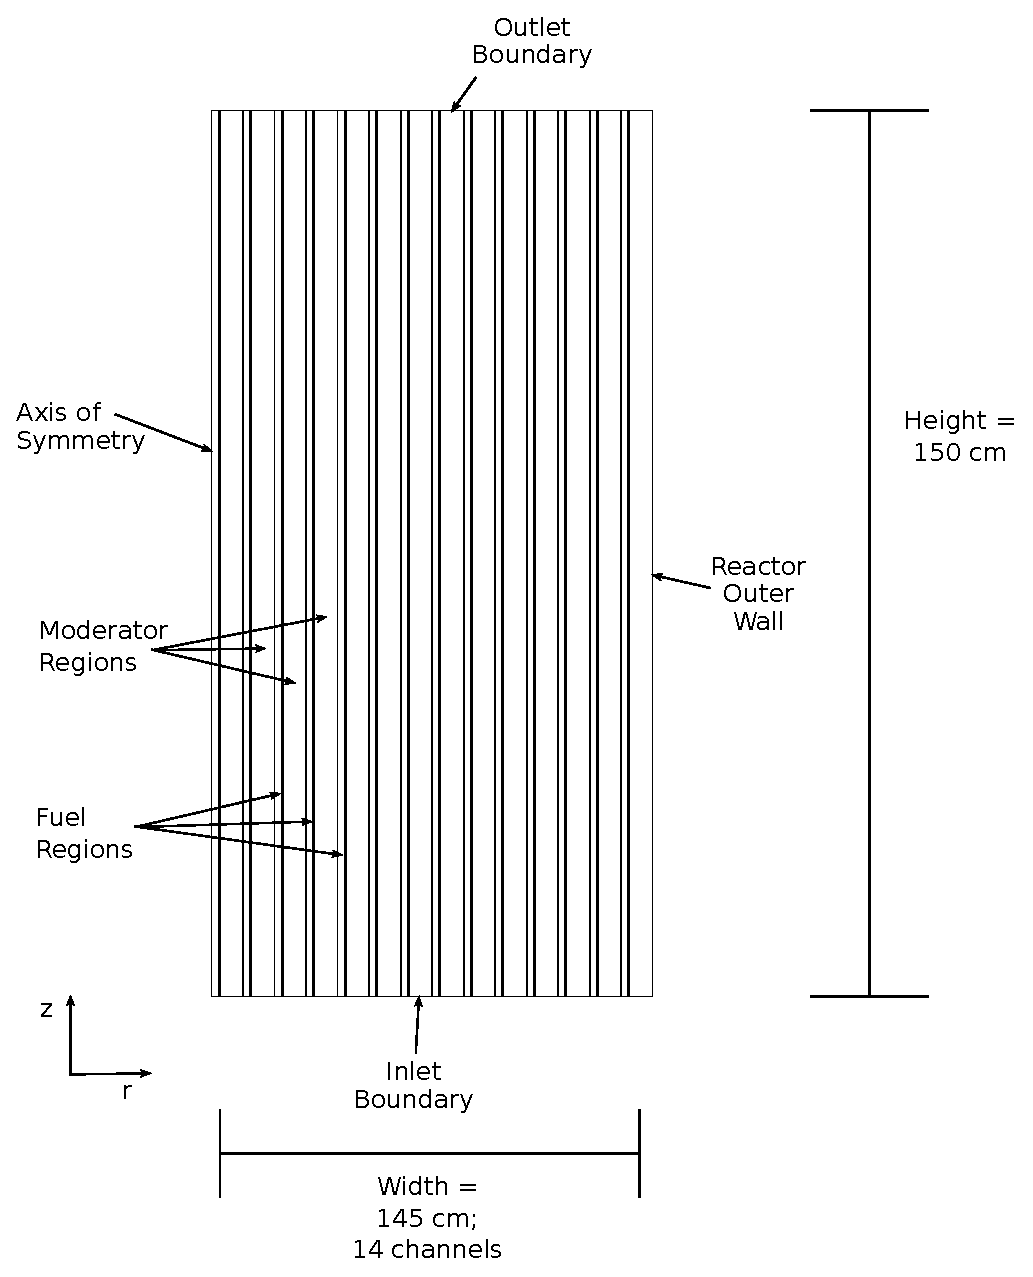
\includegraphics[width=.45\columnwidth]{msre-geometry}
	\caption{Schematic diagram of the 2D axisymmetric \gls{MSRE} geometry
	adopted by Lindsay et al. \cite{lindsay_introduction_2018}.}
	\label{fig:msre-geometry}
\end{figure}

Figure \ref{fig:msre-geometry} shows the fuel channels and moderator regions of
the 2D \gls{MSRE} geometry that Lindsay et al. adopted for their study.
They ran a two-group neutron diffusion model with six precursor groups and
vacuum boundary conditions on the outer boundaries governed by Equations
\ref{eq:neutron}, \ref{eq:precursor}, and \ref{eq:vacuum} shown in Section
\ref{sec:nts}. They modeled precursor drift due to fuel salt flow by imposing
fixed uniform flow upwards through the fuel channels shown in Figure
\ref{fig:msre-geometry}. For their thermal-hydraulics model, they employed a
governing equation for temperature in the fuel salt equivalent to Equation
\ref{eq:temp} with fixed uniform flows while also imposing a cosine-shaped heat
source term representing heat dissipation from gamma and neutron irradiation in
the graphite moderator region. In addition, all governing equations were fully
coupled and solved simultaneously as a single system of equations with implicit
Euler time-stepping to accurately and efficiently resolve the strong coupling
expected between the neutronics and temperature.

\begin{figure}[htb!]
	\centering
	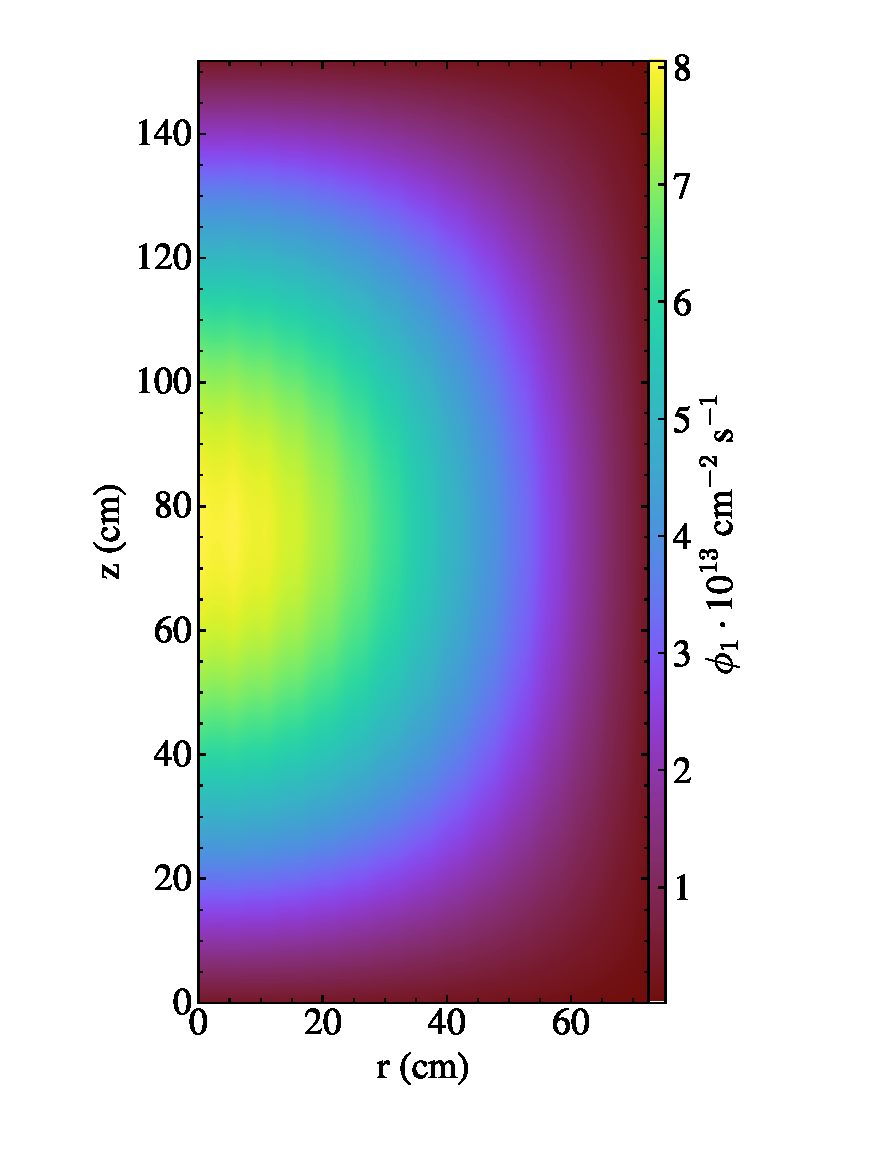
\includegraphics[width=.45\columnwidth]{2d_gamma_heating_group1}
	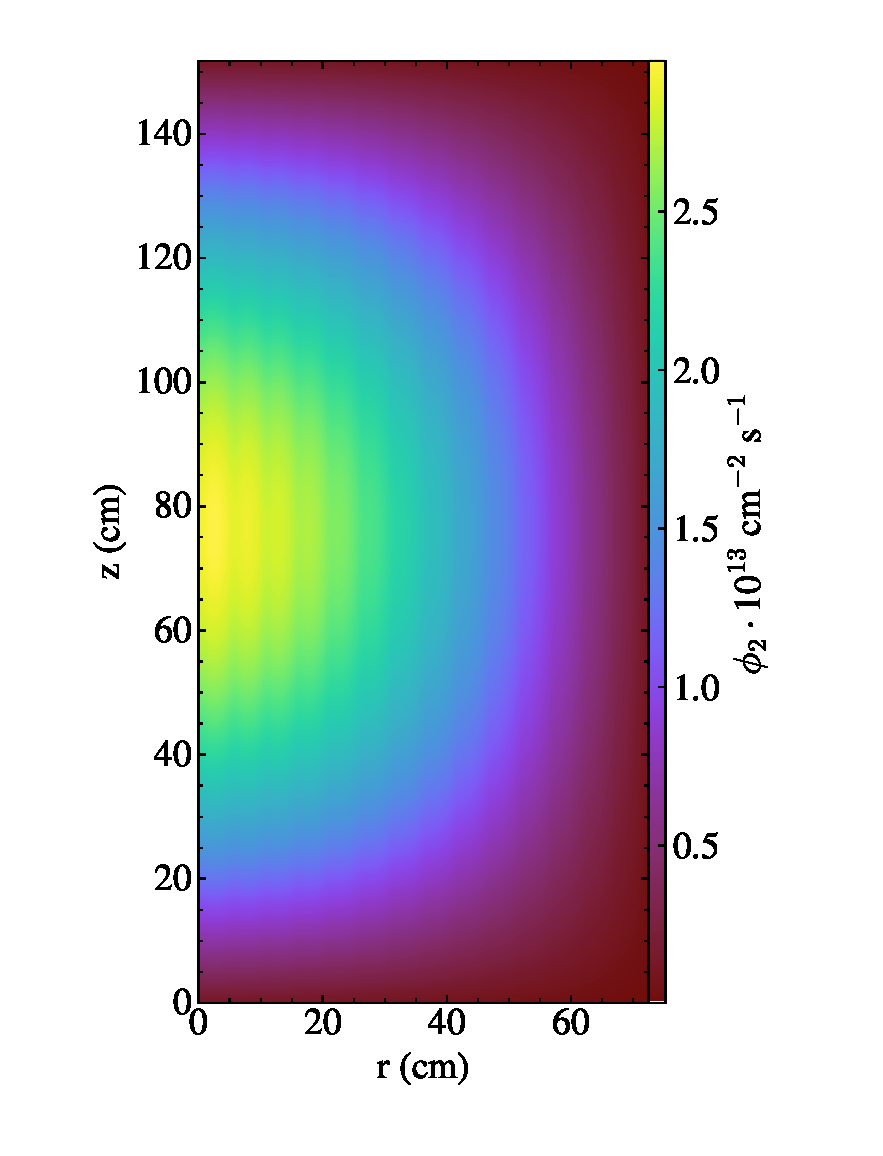
\includegraphics[width=.45\columnwidth]{2d_gamma_heating_group2}
	\caption{Neutron group 1 and 2 fluxes in the 2D axisymmetric \gls{MSRE}
	model from Lindsay et al. \cite{lindsay_introduction_2018}.}
	\label{fig:msre-flux}
\end{figure}

\begin{figure}[htb!]
	\centering
	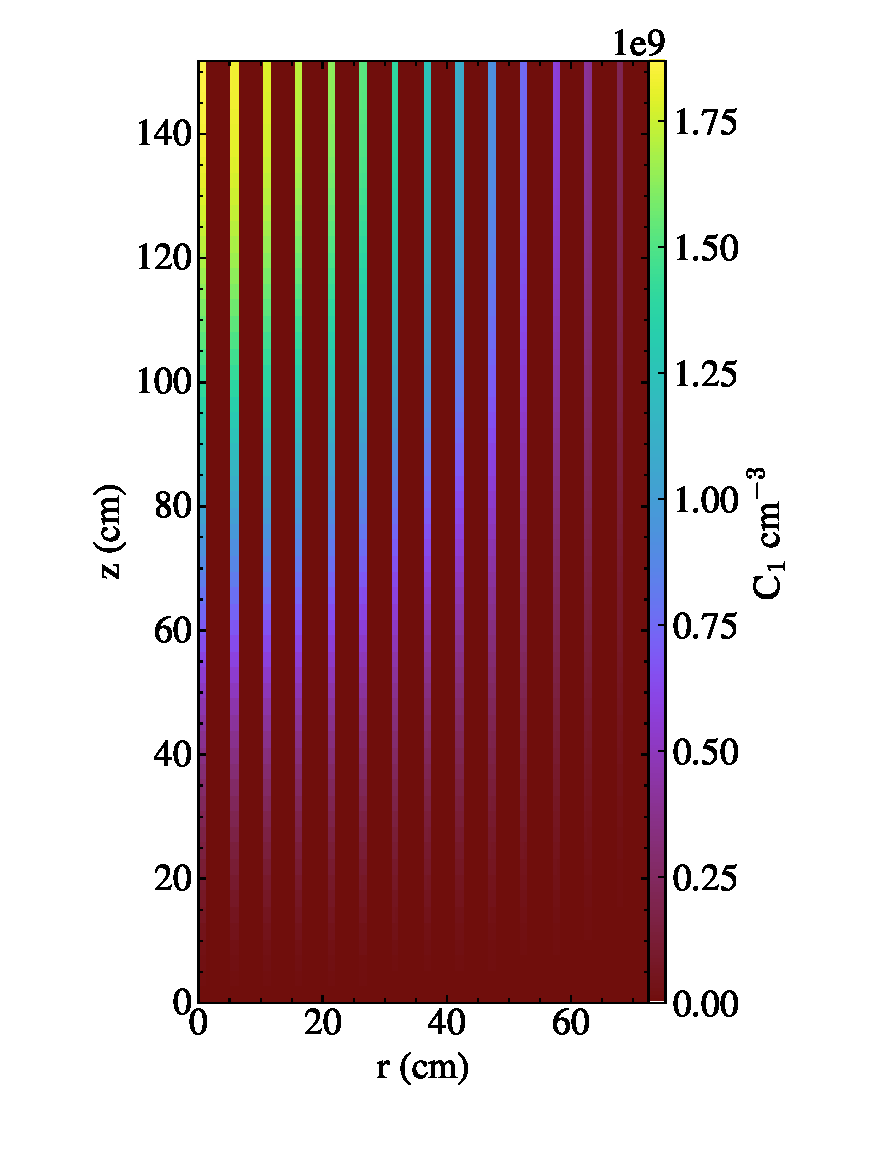
\includegraphics[width=.45\columnwidth]{2d_gamma_heating_pre1_scaled}
	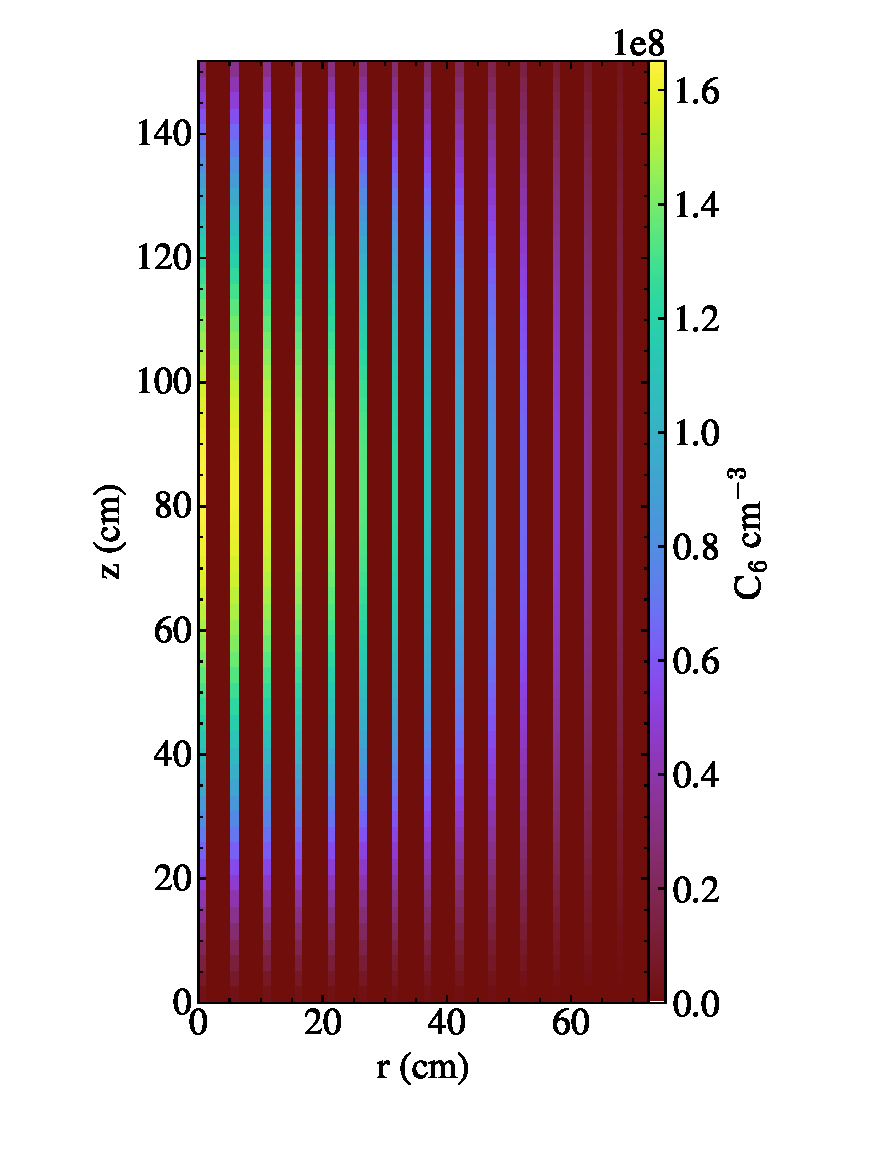
\includegraphics[width=.45\columnwidth]{2d_gamma_heating_pre6_scaled}
	\caption{Longest- and shortest-lived precursor concentrations ($\lambda =
	1.24\times 10^{-2}$s$^{-1}$ and $3.07$s${-1}$, respectively) in the 2D
	axisymmetric \gls{MSRE} model from Lindsay et al.
	\cite{lindsay_introduction_2018}.}
	\label{fig:msre-precursor}
\end{figure}

\begin{figure}[htb!]
	\centering
	\begin{minipage}[b]{0.45\columnwidth}
	    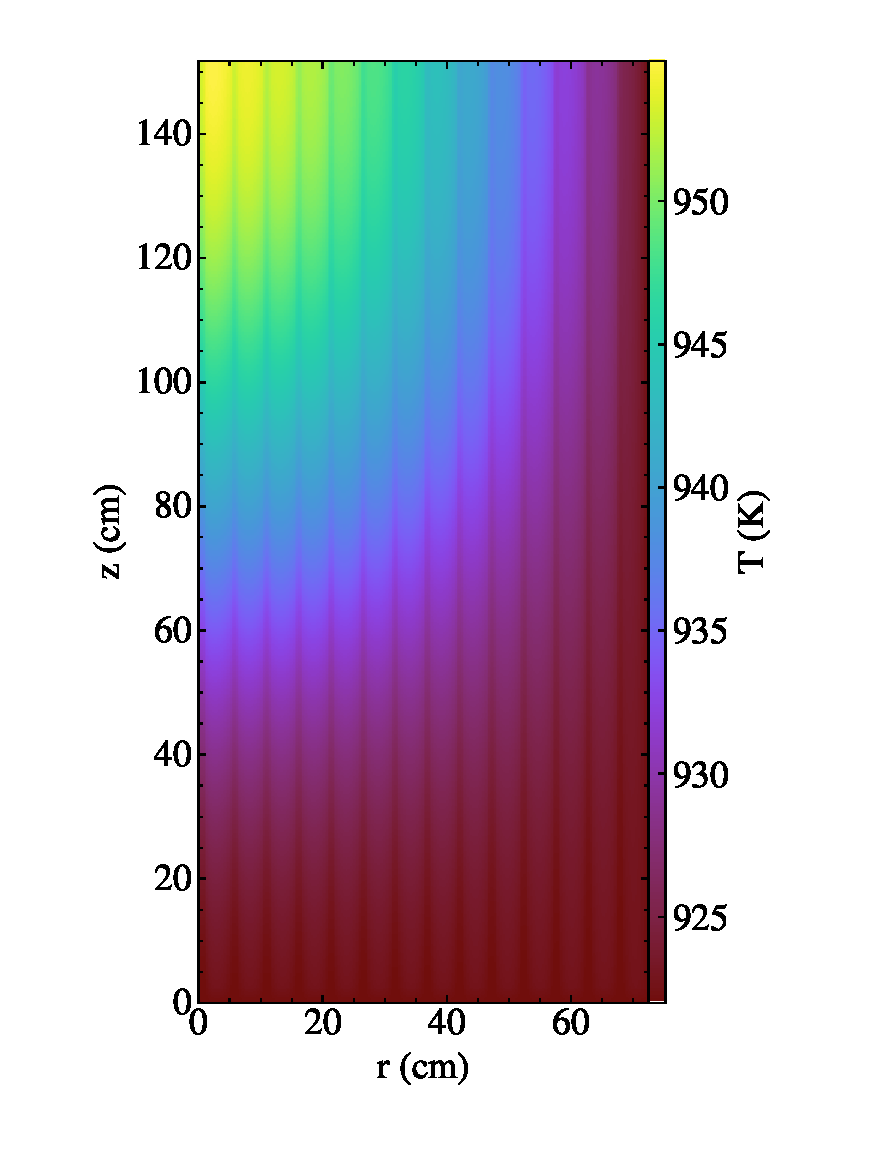
\includegraphics[width=\columnwidth]{2d_gamma_heating_temp}
	    \caption{Temperature distribution in the 2D
	    axisymmetric \gls{MSRE} model from Lindsay et al.
	    \cite{lindsay_introduction_2018}.}
	    \label{fig:msre-temp}
	\end{minipage}
	\hfill
	\begin{minipage}[b]{0.45\columnwidth}
	    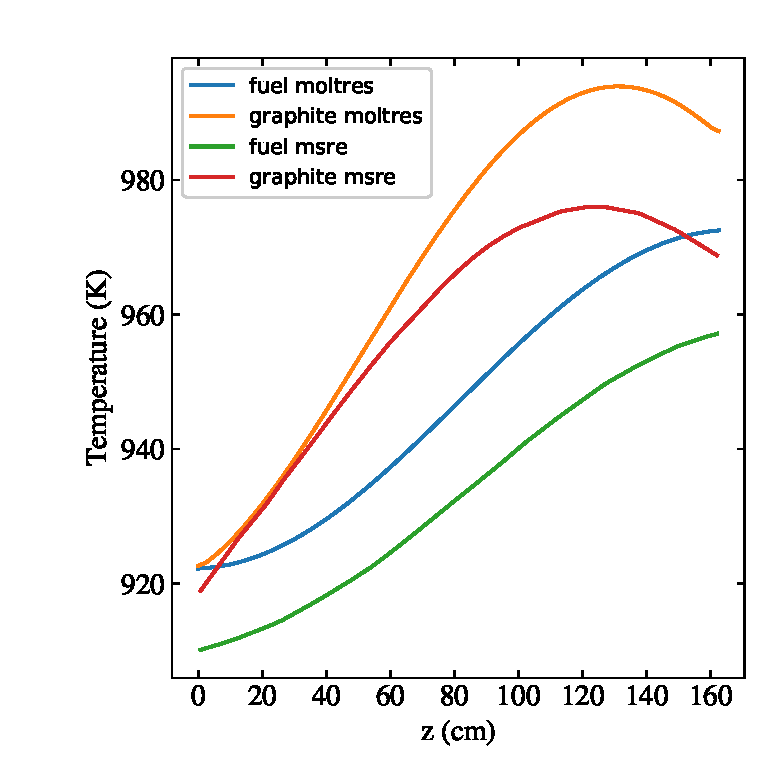
\includegraphics[width=\columnwidth]{combined_msre_moltres_axial_temps}
	    \caption{Moltres \cite{lindsay_introduction_2018} and \gls{ORNL}
	    \gls{MSRE} \cite{briggs_molten-salt_1964} axial temperature
	    distributions in the hottest fuel channel and adjacent graphite.}
	    \label{fig:msre-temp-plot}
	\end{minipage}
\end{figure}

Figure \ref{fig:msre-flux} shows the fast and thermal neutron fluxes
corresponding to group 1 and 2 in the 2D \gls{MSRE} model. As expected, the
fluxes exhibit general cosine shapes in the axial and radial directions. We
also observe minor oscillations in the radial direction coinciding with the
regular fuel and moderator lattice. The fuel regions favor the fast flux while
the moderator regions favor the thermal flux.

Figure \ref{fig:msre-precursor}
shows the longest- and shortest-lived precursor concentrations in the fuel
channels. With a long half-life of 55.9 s relative to the 6.91 s it takes for
salt to flow from bottom to top, longest-lived precursor concentration peaks
outside the model domain. By contrast, the shortest-lived precursor
concentration closely follows the cosine shape of the neutron fluxes which
dictate where the precursors are born.

Finally, Figure \ref{fig:msre-temp}
shows the temperature distribution in the 2D \gls{MSRE} model. The temperature
naturally peaks near the outlet due to upward advection. The moderator regions
experience hotter temperatures than the fuel regions due to radiative heating
and the relatively inefficiency of heat conduction in the graphite compared to
advection in the fuel salt.

\begin{figure}[htb!]
	\centering
	\begin{subfigure}[h]{0.45\columnwidth}
	    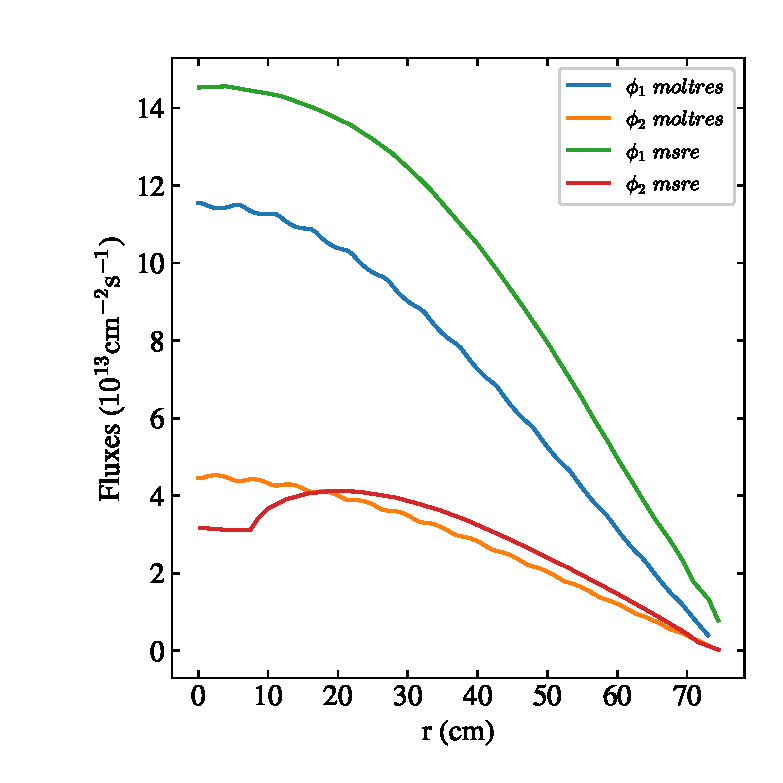
\includegraphics[width=\columnwidth]{combined_msre_moltres_radial}
	    \caption{Radial fluxes at reactor half-height.}
	    \label{fig:msre-flux-radial}
	\end{subfigure}
	\hfill
	\begin{subfigure}[h]{0.45\columnwidth}
	    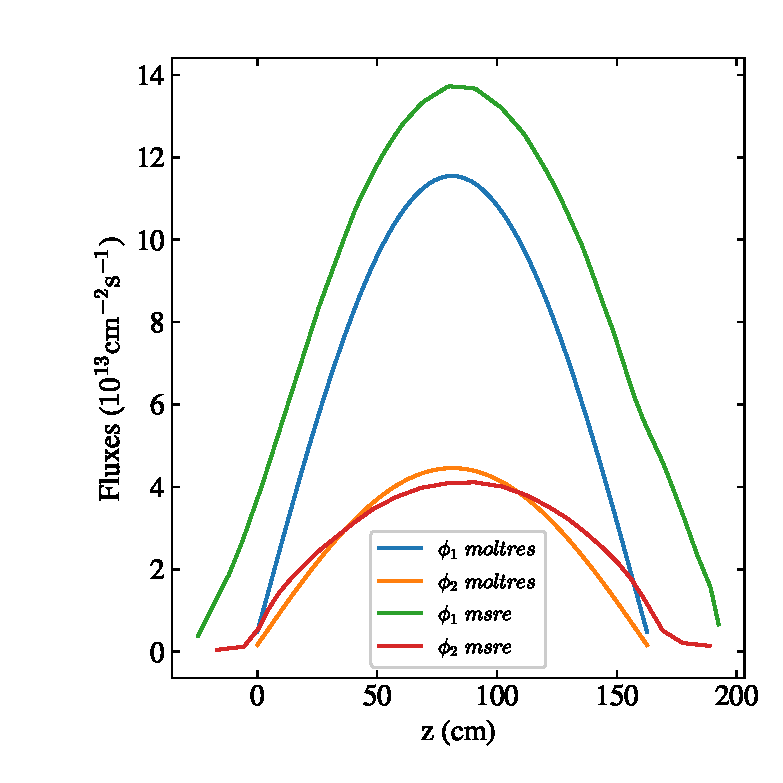
\includegraphics[width=\columnwidth]{combined_msre_moltres_axial}
	    \caption{Axial fluxes along the core centerline ($r=0$ cm).}
	    \label{fig:msre-flux-axial}
	\end{subfigure}
	\caption{The fast and thermal fluxes from
	Moltres \cite{lindsay_introduction_2018} and the \gls{ORNL} \gls{MSRE}
	design calculations \cite{briggs_molten-salt_1964}.}
\end{figure}

The corresponding neutronics and thermal-hydraulics results from their 3D model
show good qualitative agreement with the 2D results. Given the lack of
\gls{MSR} experimental data, they compared their 2D model results with
\gls{MSRE} design calculations performed using legacy software in 1963-1964 at
\gls{ORNL}. Their neutron flux and temperature distribution results showed good
qualitative agreement with \gls{ORNL} data. The authors attributed
discrepancies to the following differences in the two modeling approaches: the
absence of axial heat conduction and the use of 32 neutron groups in the
\gls{ORNL} calculations, and the exclusion of control rod thimbles in the
Moltres calculations.

\subsubsection{Critical Assessment} \label{sec:msre-critique}

Lindsay et al.'s work illustrated early development efforts for neutronics and thermal-hydraulics
models in Moltres and demonstrated, along with advanced capabilities from the \gls{MOOSE}
framework, fully-coupled simulations of the \gls{MSRE} with implicit time-stepping. The
decent qualitative agreement observed between Moltres and the \gls{ORNL}
\gls{MSRE} calculations proved that Moltres was capable of simulating
\glspl{MSR} under some simplifying assumptions.

On the other hand, significant improvements could be made to Moltres to better
model multiphysics phenomena in \glspl{MSR}. For instance, replacing the
fixed uniform salt flow with a proper flow profile governed by fluid flow
equations would accurately capture precursor and temperature advection.
Temperature advection has a particularly large impact on the temperature
distribution in the fuel salt since molten salts generally have large Prandtl
numbers, which measures the ratio of convective to conductive heat transfer.
The flow-modeling feature would be of even greater importance when modeling
pool-type \glspl{MSR} which consist of a single large fuel salt region in the
reactor core.

Another essential feature for modeling \glspl{MSR}, which was already under
development at the time of publication, is a precursor loop
system to recirculate precursors back into the core. While some precursors
decay outside the core, others survive long enough to recirculate back into the
core. The loop system would provide a more accurate estimate of the delayed
neutron fraction as opposed to discarding all precursors which flowed out of
the core. In transient simulations involving sudden increases in the neutron
flux, precursors recirculating into the core can induce observable jumps and
dips in the power output due to the associated reactivity insertion from the
delayed neutrons.

Additionally, Moltres would also benefit from a decay heat model which Lindsay
et al. also mentioned in their work \cite{lindsay_introduction_2018},
especially for accident transient analyses. While decay heat from fission
product decays represents a small fraction ($\sim5\%$) of total power output,
this heat source can be significant in unprotected loss of flow or loss of
secondary cooling accidents. Therefore, understanding residual heat generation
from fission product decays in \gls{MSR} is essential in preventing further
structural failure in the aftermath of an accident.

Specific to reactor physics modeling, Moltres also requires an accurate method for modeling
control rods. As observed in Figure \ref{fig:msre-flux}, the omission of control rods led to the
significant discrepancies in the thermal flux distribution. However, developing control rod
modeling capability in Moltres is nontrivial given that neutron diffusion theory performs poorly
within highly neutron-absorbing regions.

Lastly, the authors recognized two other avenues for future work: more
rigorous validation and verification of Moltres' capabilities by comparison
with more detailed experimental data and other modern \gls{MSR} modeling
efforts; and the study of transient simulation cases such as control rod
ejection, single channel blockage, loss of flow, and loss of secondary cooling.

\subsection{Advancements in Moltres and Transient Simulations of the MSFR}
\label{sec:msfr}

This section follows my previous work for my Master's degree in \textit{Advancement and
Verification of Moltres for Molten Salt Reactor Safety Analysis} \cite{park_advancement_2020},
which I shall refer to as ``this work'' in this subsection.

This work represents a continuation of the work by Lindsay et al.
\cite{lindsay_introduction_2018} in the development of Moltres as an \gls{MSR}
simulation tool. New features introduced include the coupling of the existing
neutronics and temperature equations to incompressible Navier-Stokes equations
to model flow dynamics, the precursor loop system, and the decay heat model.
I later demonstrated these features through steady-state and transient
simulations of a 2D axisymmetric \gls{MSFR} model.

Moltres couples natively with the \texttt{Navier-Stokes} module in \gls{MOOSE} for
incompressible flow modeling capabilities. Efforts towards coupling
the neutronics capabilities to the \texttt{Navier-Stokes} module were already
underway during the peer review process of the work described in Section
\ref{sec:msre}. Section \ref{sec:th} describes the governing equations for
incompressible flow and temperature advection-diffusion. At the same time,
the precursor loop system was being developed to model
precursor recirculation into the core. The precursor loop system leverages on
the \texttt{MultiApp} system in \gls{MOOSE} to couple a 1D pipe model to the
core to simulate precursor flow outside the core. The core and the pipe models
are coupled via inlet and outlet boundary conditions, as detailed in Section
\ref{sec:moltres-loop}. The loop system can also accommodate a pointwise heat
exchanger model with heat removal rate as a function of time
and/or auxiliary variables in the Moltres simulation.

In addition, I developed a decay heat model to simulate delayed heat release
from the decay of fission products, similar to delayed neutron emission
from precursors. The decay heat model introduces decay heat groups of different
decay constants, variables representing the decay heat groups, and modifies the
heat source term given by Equation \ref{eq:heat-source} to account for
the delayed heat generation. 

The number of decay heat groups and their respective decay constants depends on
the decay heat profile of the reactor after a specified period of operation.
Determining the decay heat profile requires fuel depletion calculations to
obtain the fuel composition during/after reactor operation and subsequent
calculations for the cumulative decay heat released from individual isotopes.
In this work, I cited results by Aufiero et al. \cite{aufiero_extended_2013}
who determined that three decay heat groups ($J=3$) were sufficient to
reproduce the decay heat profile of the \gls{MSFR} equilibrium fuel composition
for up to 300 seconds after shutdown with a relative error of less than 2\%.

\begin{figure}[htb!]
	\centering
	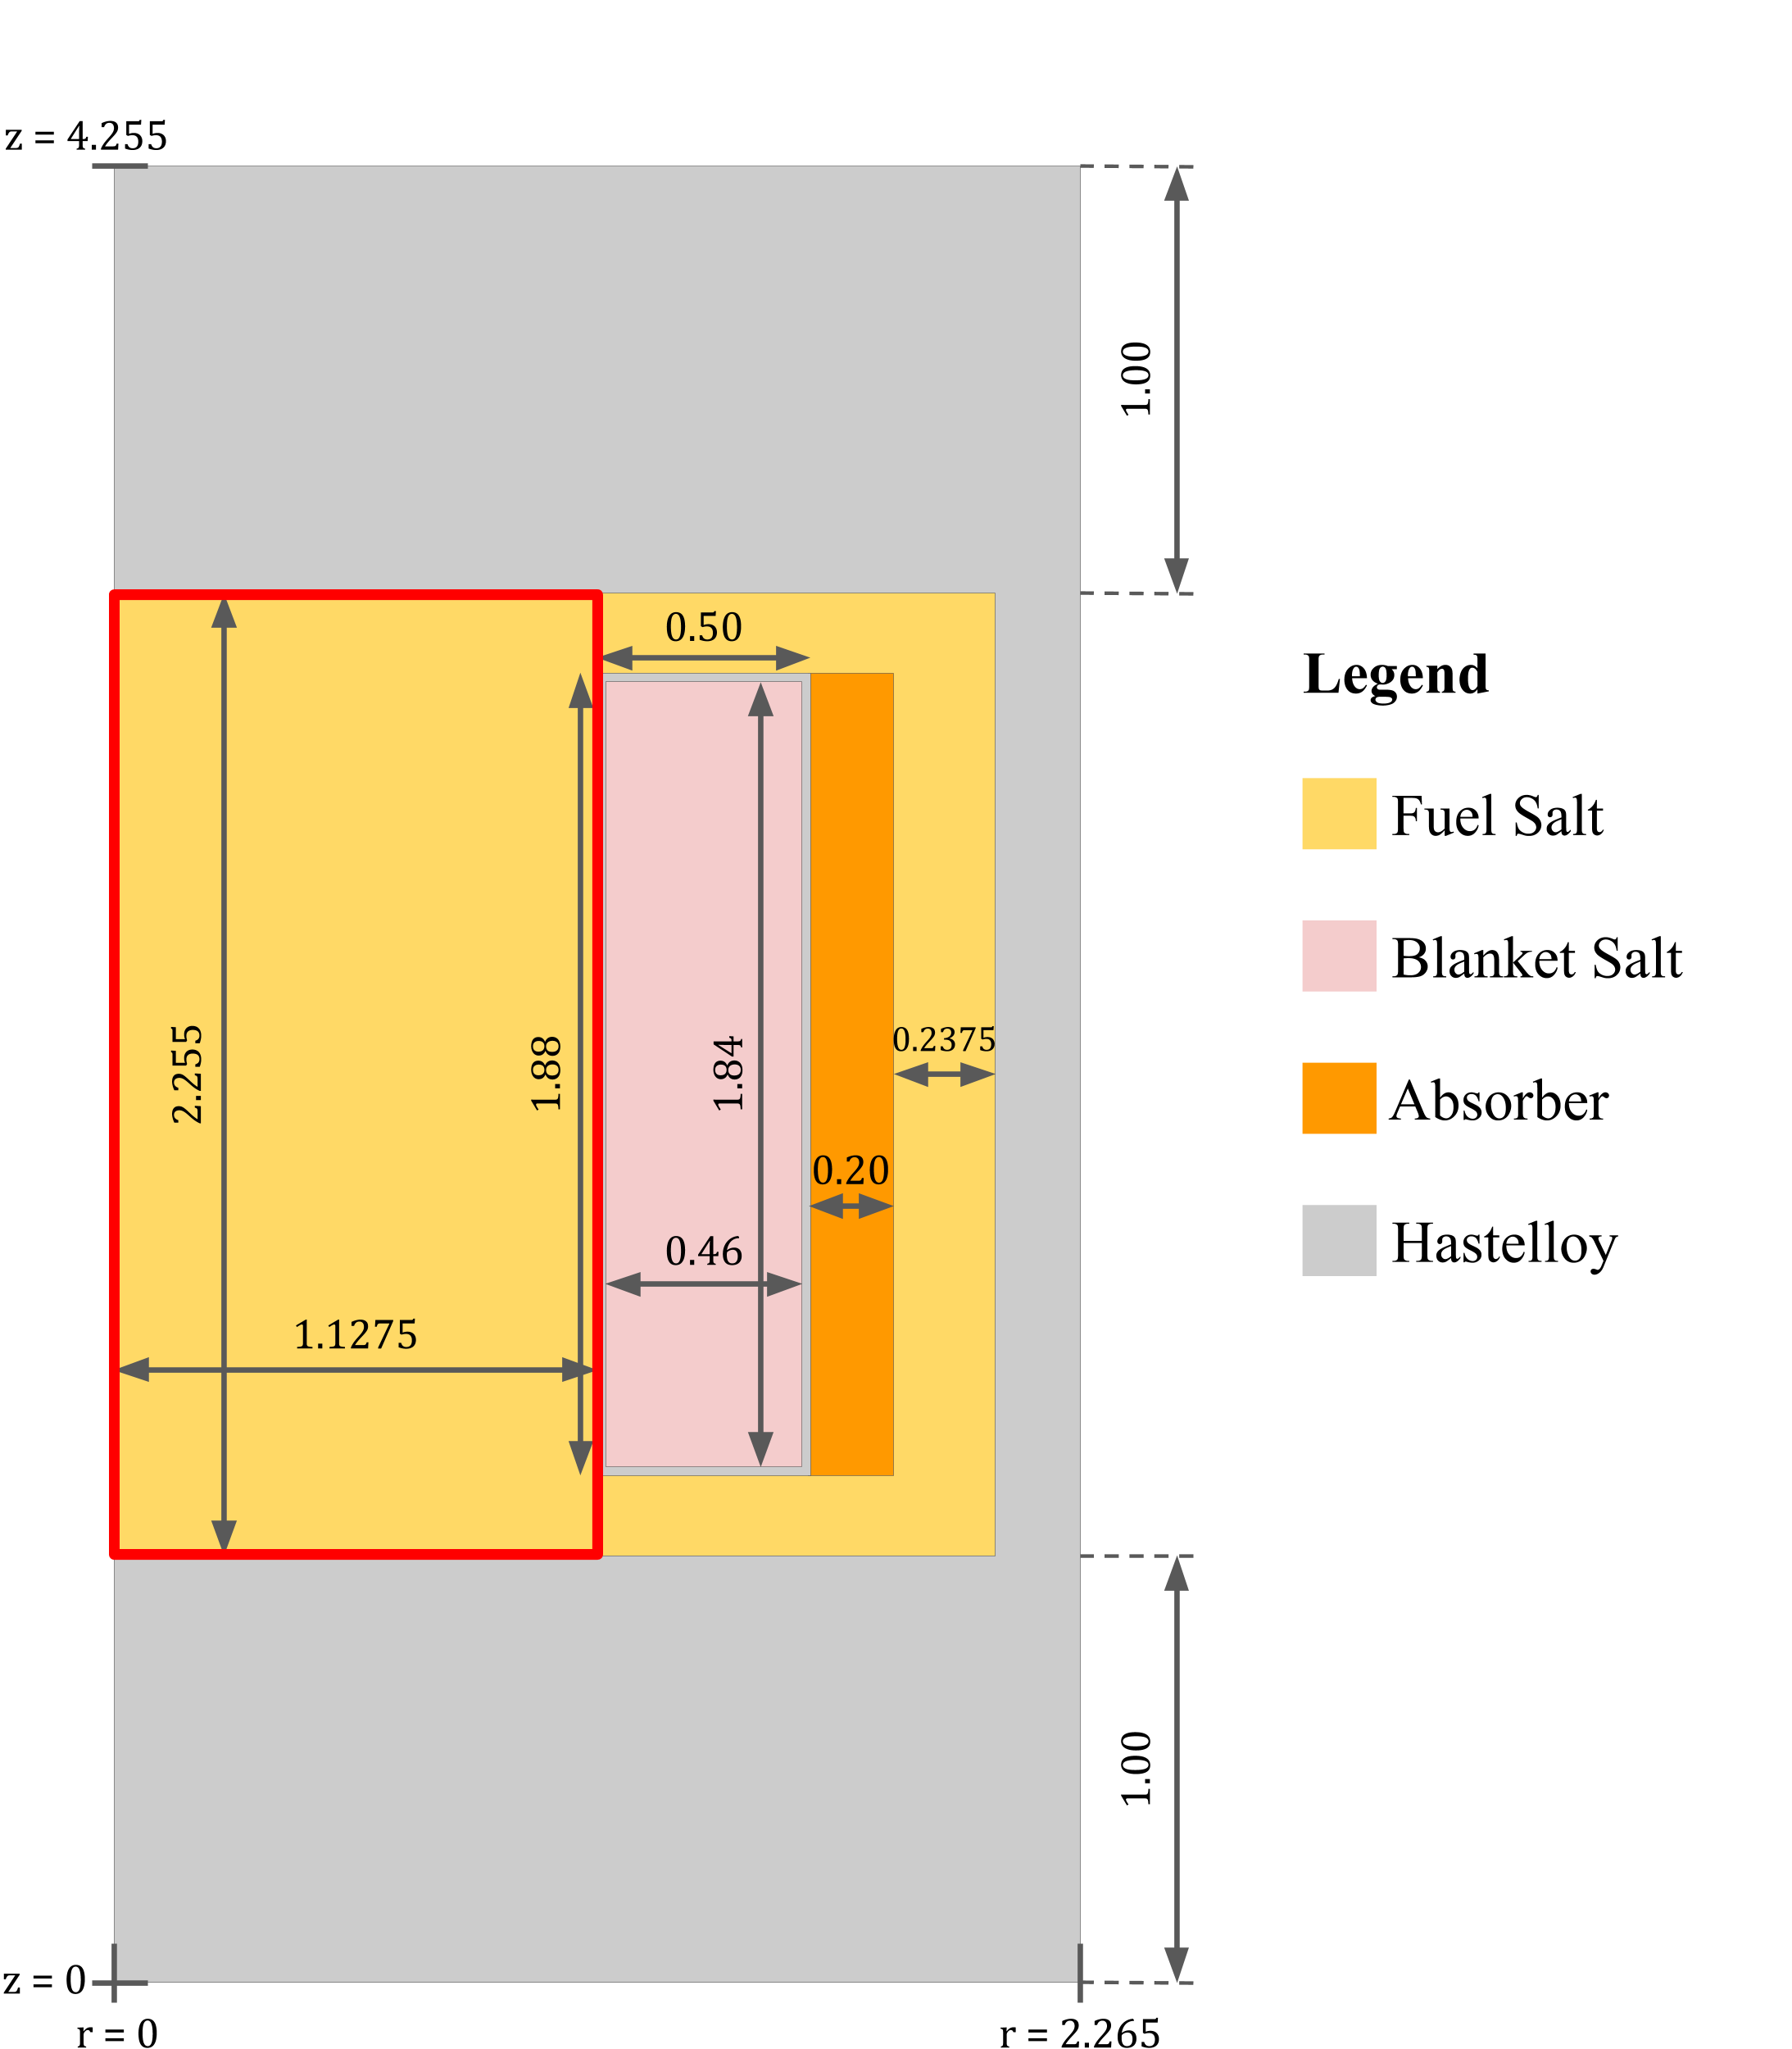
\includegraphics[width=.55\columnwidth]{central-core-legend}
	\caption{Schematic diagram of the 2D axisymmetric \gls{MSFR} model with
	the core region enclosed by the red box \cite{park_advancement_2020}.}
	\label{fig:msfr-geometry}
\end{figure}

For the verification and demonstration of the capabilities introduced in this
work, I ran coupled, steady-state and unprotected accident transient
simulations of the \gls{MSFR} and compared the results with published results
by Fiorina et al. \cite{fiorina_modelling_2014} and Aufiero et al.
\cite{aufiero_development_2014}. The PoliMi and TU Delft models in this section
refer to two sets of results published by Fiorina et al. I compensated for
the lack of a turbulence model in Moltres by imposing a fixed turbulent
viscosity of 40 Pa$\cdot$s in addition to the molecular viscosity $\mu$ in
Equation \ref{eq:momemtum}. Figure \ref{fig:msfr-geometry} shows the 2D
axisymmetric \gls{MSFR} model with the core region indicated with the red box,
while the rest of the fuel region was modeled with the 1D loop system. Fuel
salt flows into the core region from the inlet at the bottom-right corner and
out through the outlet at the top-right corner.

\begin{figure}[htb!]
    \centering
    \begin{subfigure}[t]{.35\textwidth}
        \centering
        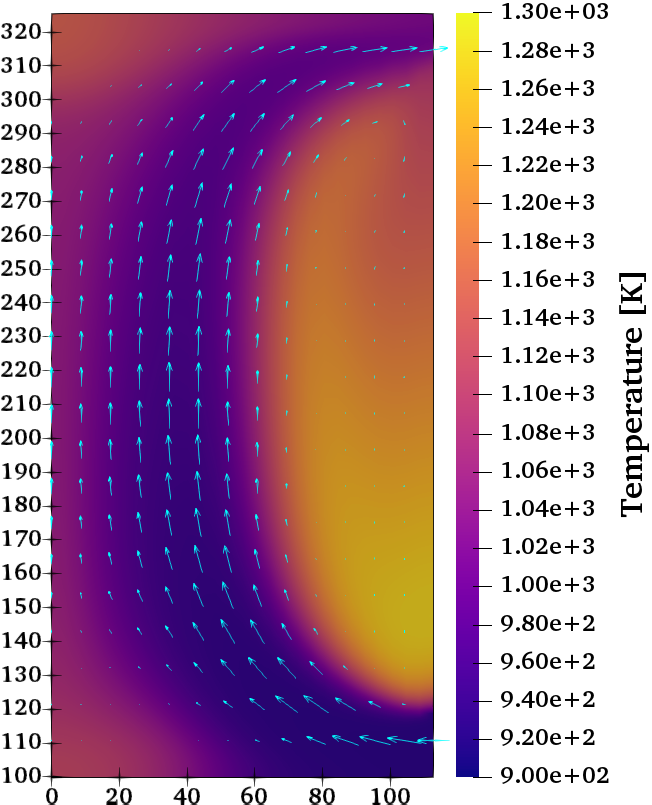
\includegraphics[width=\textwidth]{flow-temp-plasma}
    \end{subfigure}
    \hfill
    \begin{subfigure}[t]{.625\textwidth}
        \centering
        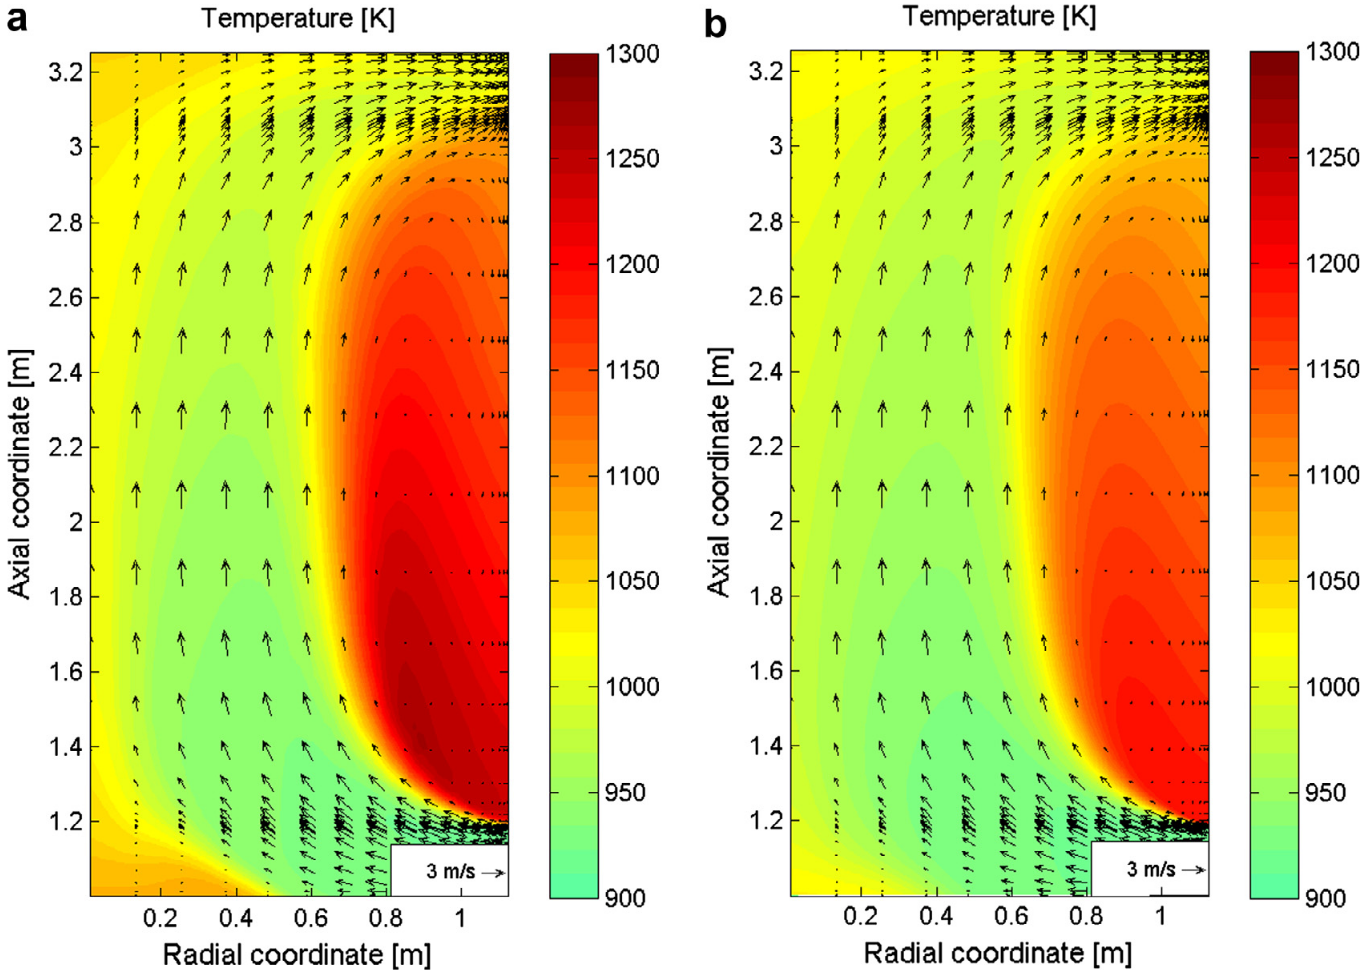
\includegraphics[width=\textwidth]{flow-temp-fiorina}
    \end{subfigure}
    \caption{Temperature and velocity fields in the core from Moltres
    (left), PoliMi (center), and TU Delft (right) models. The colors represent
    temperature according to the respective color bars and the arrows
    represent velocity fields. \cite{park_advancement_2020}}
    \label{fig:flow-temp}
\end{figure}

Figure \ref{fig:flow-temp} shows the steady-state temperature and velocity
fields in the core from the Moltres, PoliMi, and TU Delft models. The Moltres
model showed
good qualitative agreement with the PoliMi and TU Delft models as the plots
show similar flow and hotspot features in all three models. The salt flow
largely follows a parabolic path from the inlet to the outlet. A large
recirculation region formed near the right wall while the top and bottom
regions along the central axis experience relatively stagnant flow compared to
the main salt flowstream. The temperature hotspots coincide with the regions of
recirculation and stagnation because convection is the dominant heat transfer
mechanism. Maximum temperatures are observed near the bottom of the
recirculation zones; the Moltres model reports 1275 K which is closer to the
PoliMi model ($\sim1300$ K) than the TU Delft model ($\sim1200$ K). Thus, the
incompressible flow model in Moltres performed well in reproducing the
thermal-hydraulic profiles of the \gls{MSFR} under steady state conditions in
spite of the fixed turbulent viscosity assumption.

\begin{figure}[b!]
    \centering
    \begin{subfigure}[t]{.30\textwidth}
        \centering
        \vspace{.9cm}
        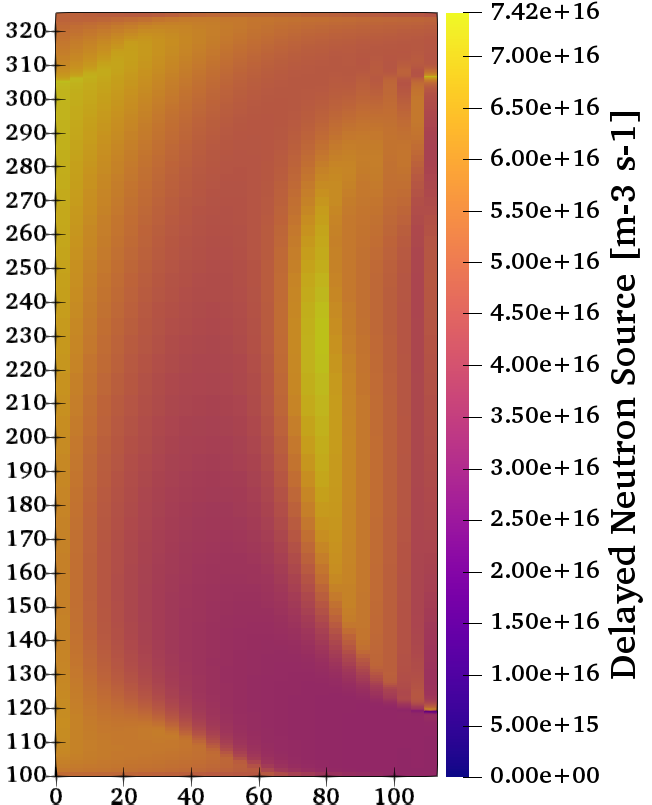
\includegraphics[width=\textwidth]{pre}
    \end{subfigure}
    \begin{subfigure}[t]{.69\textwidth}
        \centering
        \vspace{0pt}
        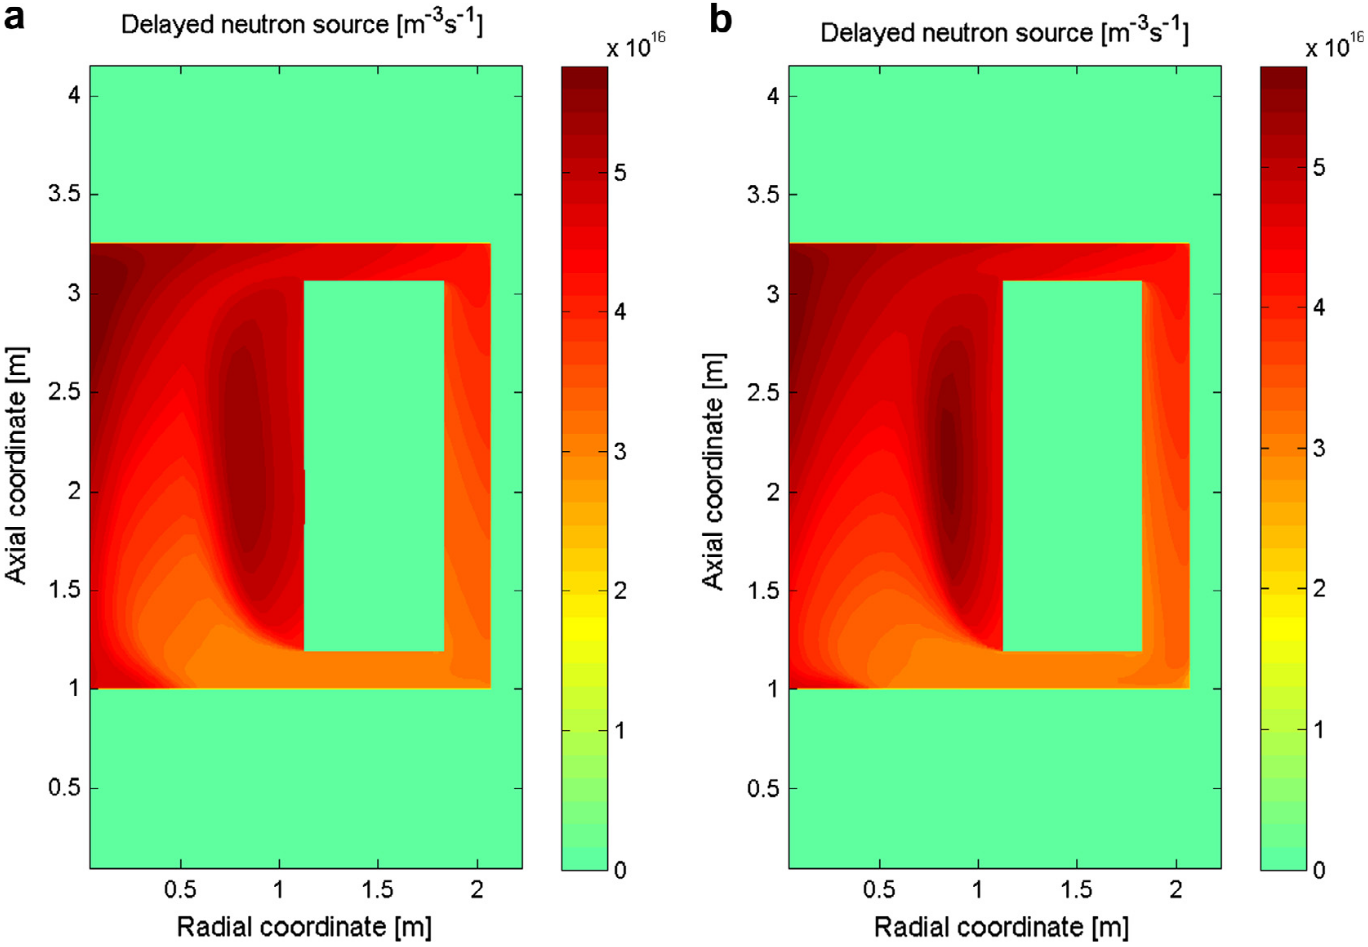
\includegraphics[width=\textwidth]{fiorina-pre}
    \end{subfigure}
    \caption{Total delayed neutron source distribution in the core from the
    Moltres (left), PoliMi (center), and TU Delft (right) models.}
    \label{fig:pre}
\end{figure}

Moltres reported a peak total neutron flux of $9.80 \times 10^{15}$
cm$^{-2}\cdot$s$^{-1}$ which is close to the 8.6 and 9.0 $\times 10^{15}$
cm$^{-2}\cdot$s$^{-1}$ values reported by Fiorina et al.
\cite{fiorina_molten_2013} and \cite{aufiero_development_2014}. However, the
delayed neutron source distribution from the Moltres model exhibits some
differences compared to the PoliMi and TU Delft models as shown in Figure
\ref{fig:pre}. The Moltres model retains fewer precursors than the other two
models, resulting in a higher 44.16\% out-of-core delayed neutron emissions
compared with the 34.80\% and 34.85\% from the other models
\cite{park_advancement_2020}. Therefore, the incompressible flow model with
constant turbulent viscosity fell short on accurately capturing precursor
drift in the \gls{MSFR}.

\begin{figure}[htb]
    \centering
    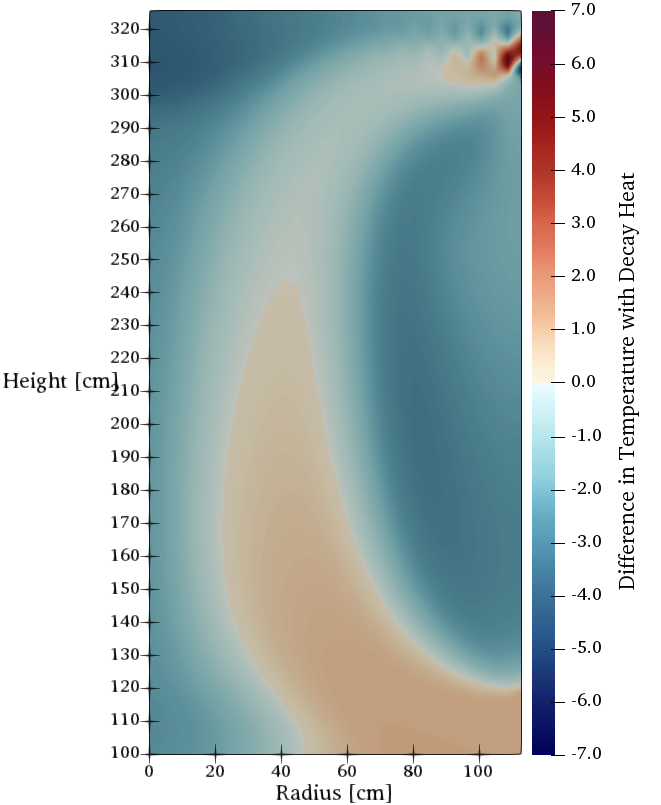
\includegraphics[width=.5\textwidth]{decay-heat-temp}
    \caption{Difference in core temperatures at steady-state with decay heat
    relative to the result without decay heat (Figure \ref{fig:flow-temp}).}
    \label{fig:decayheattemp}
\end{figure}

This work also compared steady-state temperature distributions with and without
the decay heat model. As expected, the decay heat model effectively flattens
the heat source distribution, causing a reduction in the maximum
temperatures and an increase in the minimum temperatures observed in the model.
Figure \ref{fig:decayheattemp} shows a decrease in temperature in the hotspot
regions and an increase in temperature near the inlet which is the coolest
region in the core.

For the transient studies, this work considered unprotected reactivity
insertion, loss of heat sink, loss of flow, and pump overspeed accidents. The
term ``unprotected'' signifies accident scenarios without reactor SCRAM.
Moltres reproduced similar trends observed in the PoliMi and TU Delft
models for the reactivity insertion and loss of heat sink scenarios. For
instance, Figure \ref{fig:200pcmheat} shows the power output response of the
three models following a 200 pcm step reactivity insertion. The lower peak from
the Moltres model is attributed to the more strongly negative fuel temperature
reactivity feedback coefficient of $-7.184$ pcm$\cdot$K$^{-1}$ compared to
approximately $-6.5$ pcm$\cdot$K$^{-1}$ for the PoliMi and TU Delft models.

\begin{figure}[htb!]
    \centering
    \begin{subfigure}[b]{.49\textwidth}
      \centering
      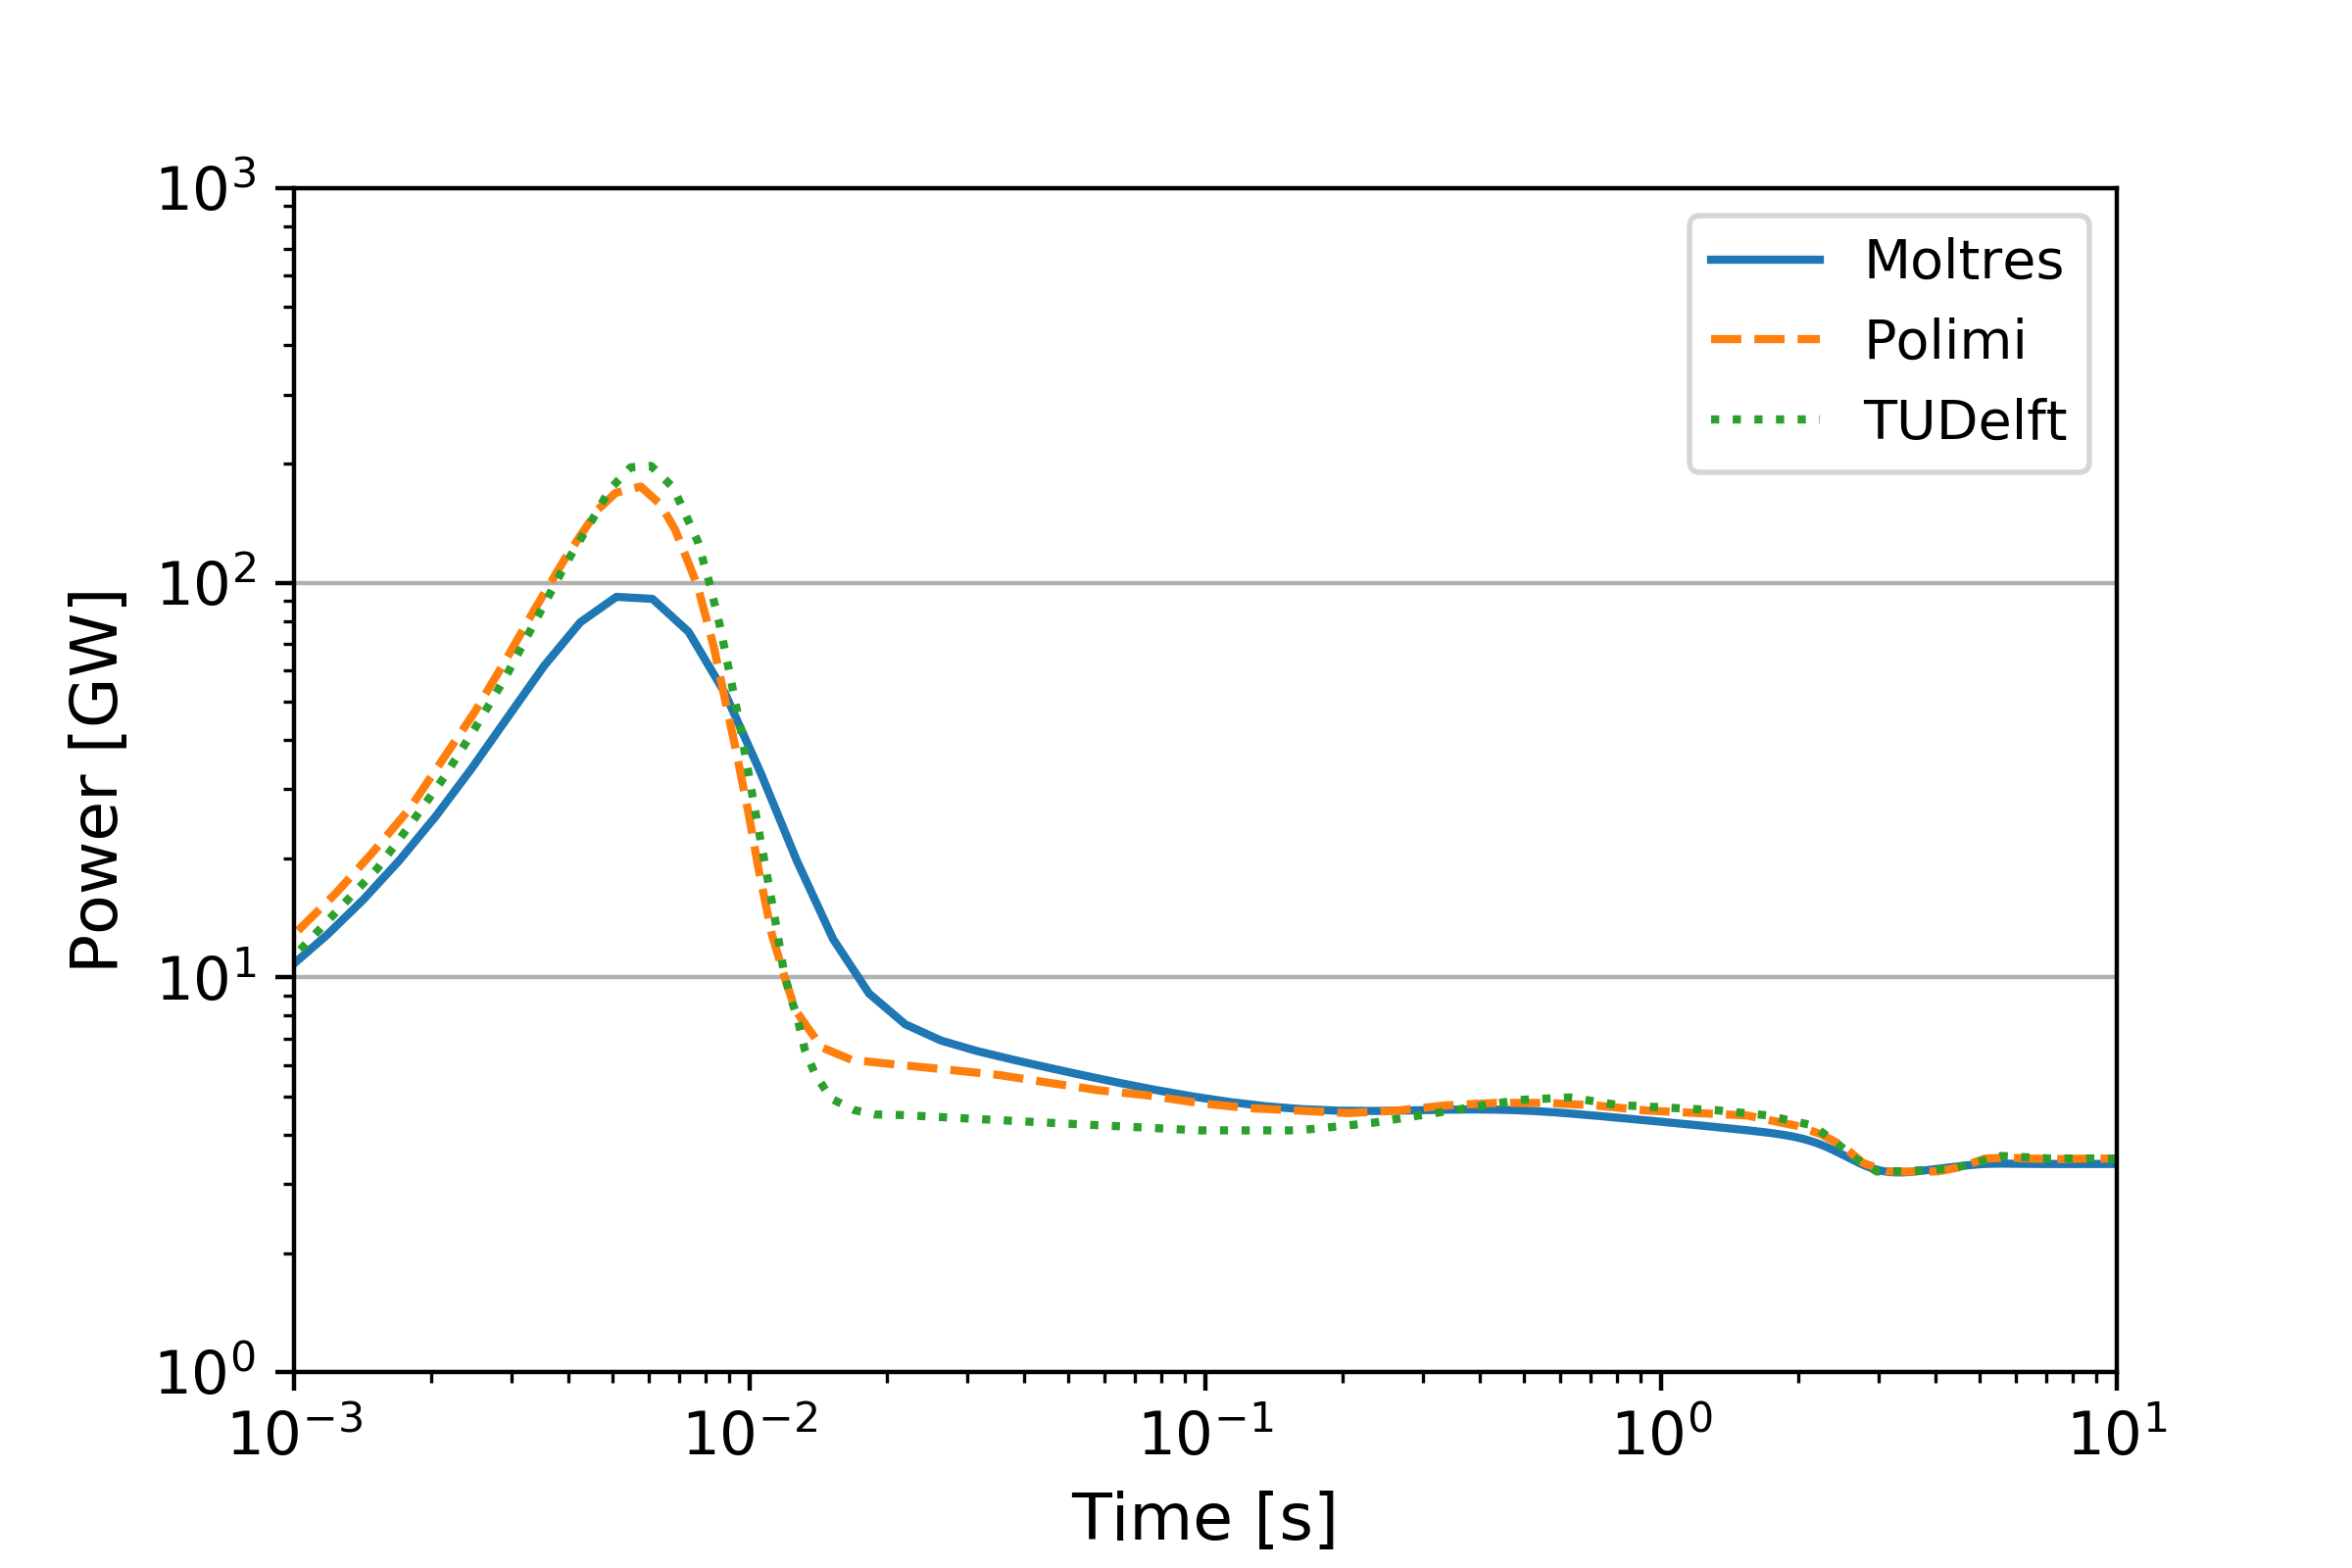
\includegraphics[width=\textwidth]{200pcm-heat}
      \caption{Power output following a 200 pcm step-wise unprotected reactivity
        insertion in the Moltres, PoliMi, and
        TU Delft models \cite{fiorina_modelling_2014}.}
      \label{fig:200pcmheat}
    \end{subfigure}
    \hfill
    \begin{subfigure}[b]{.49\textwidth}
      \centering
      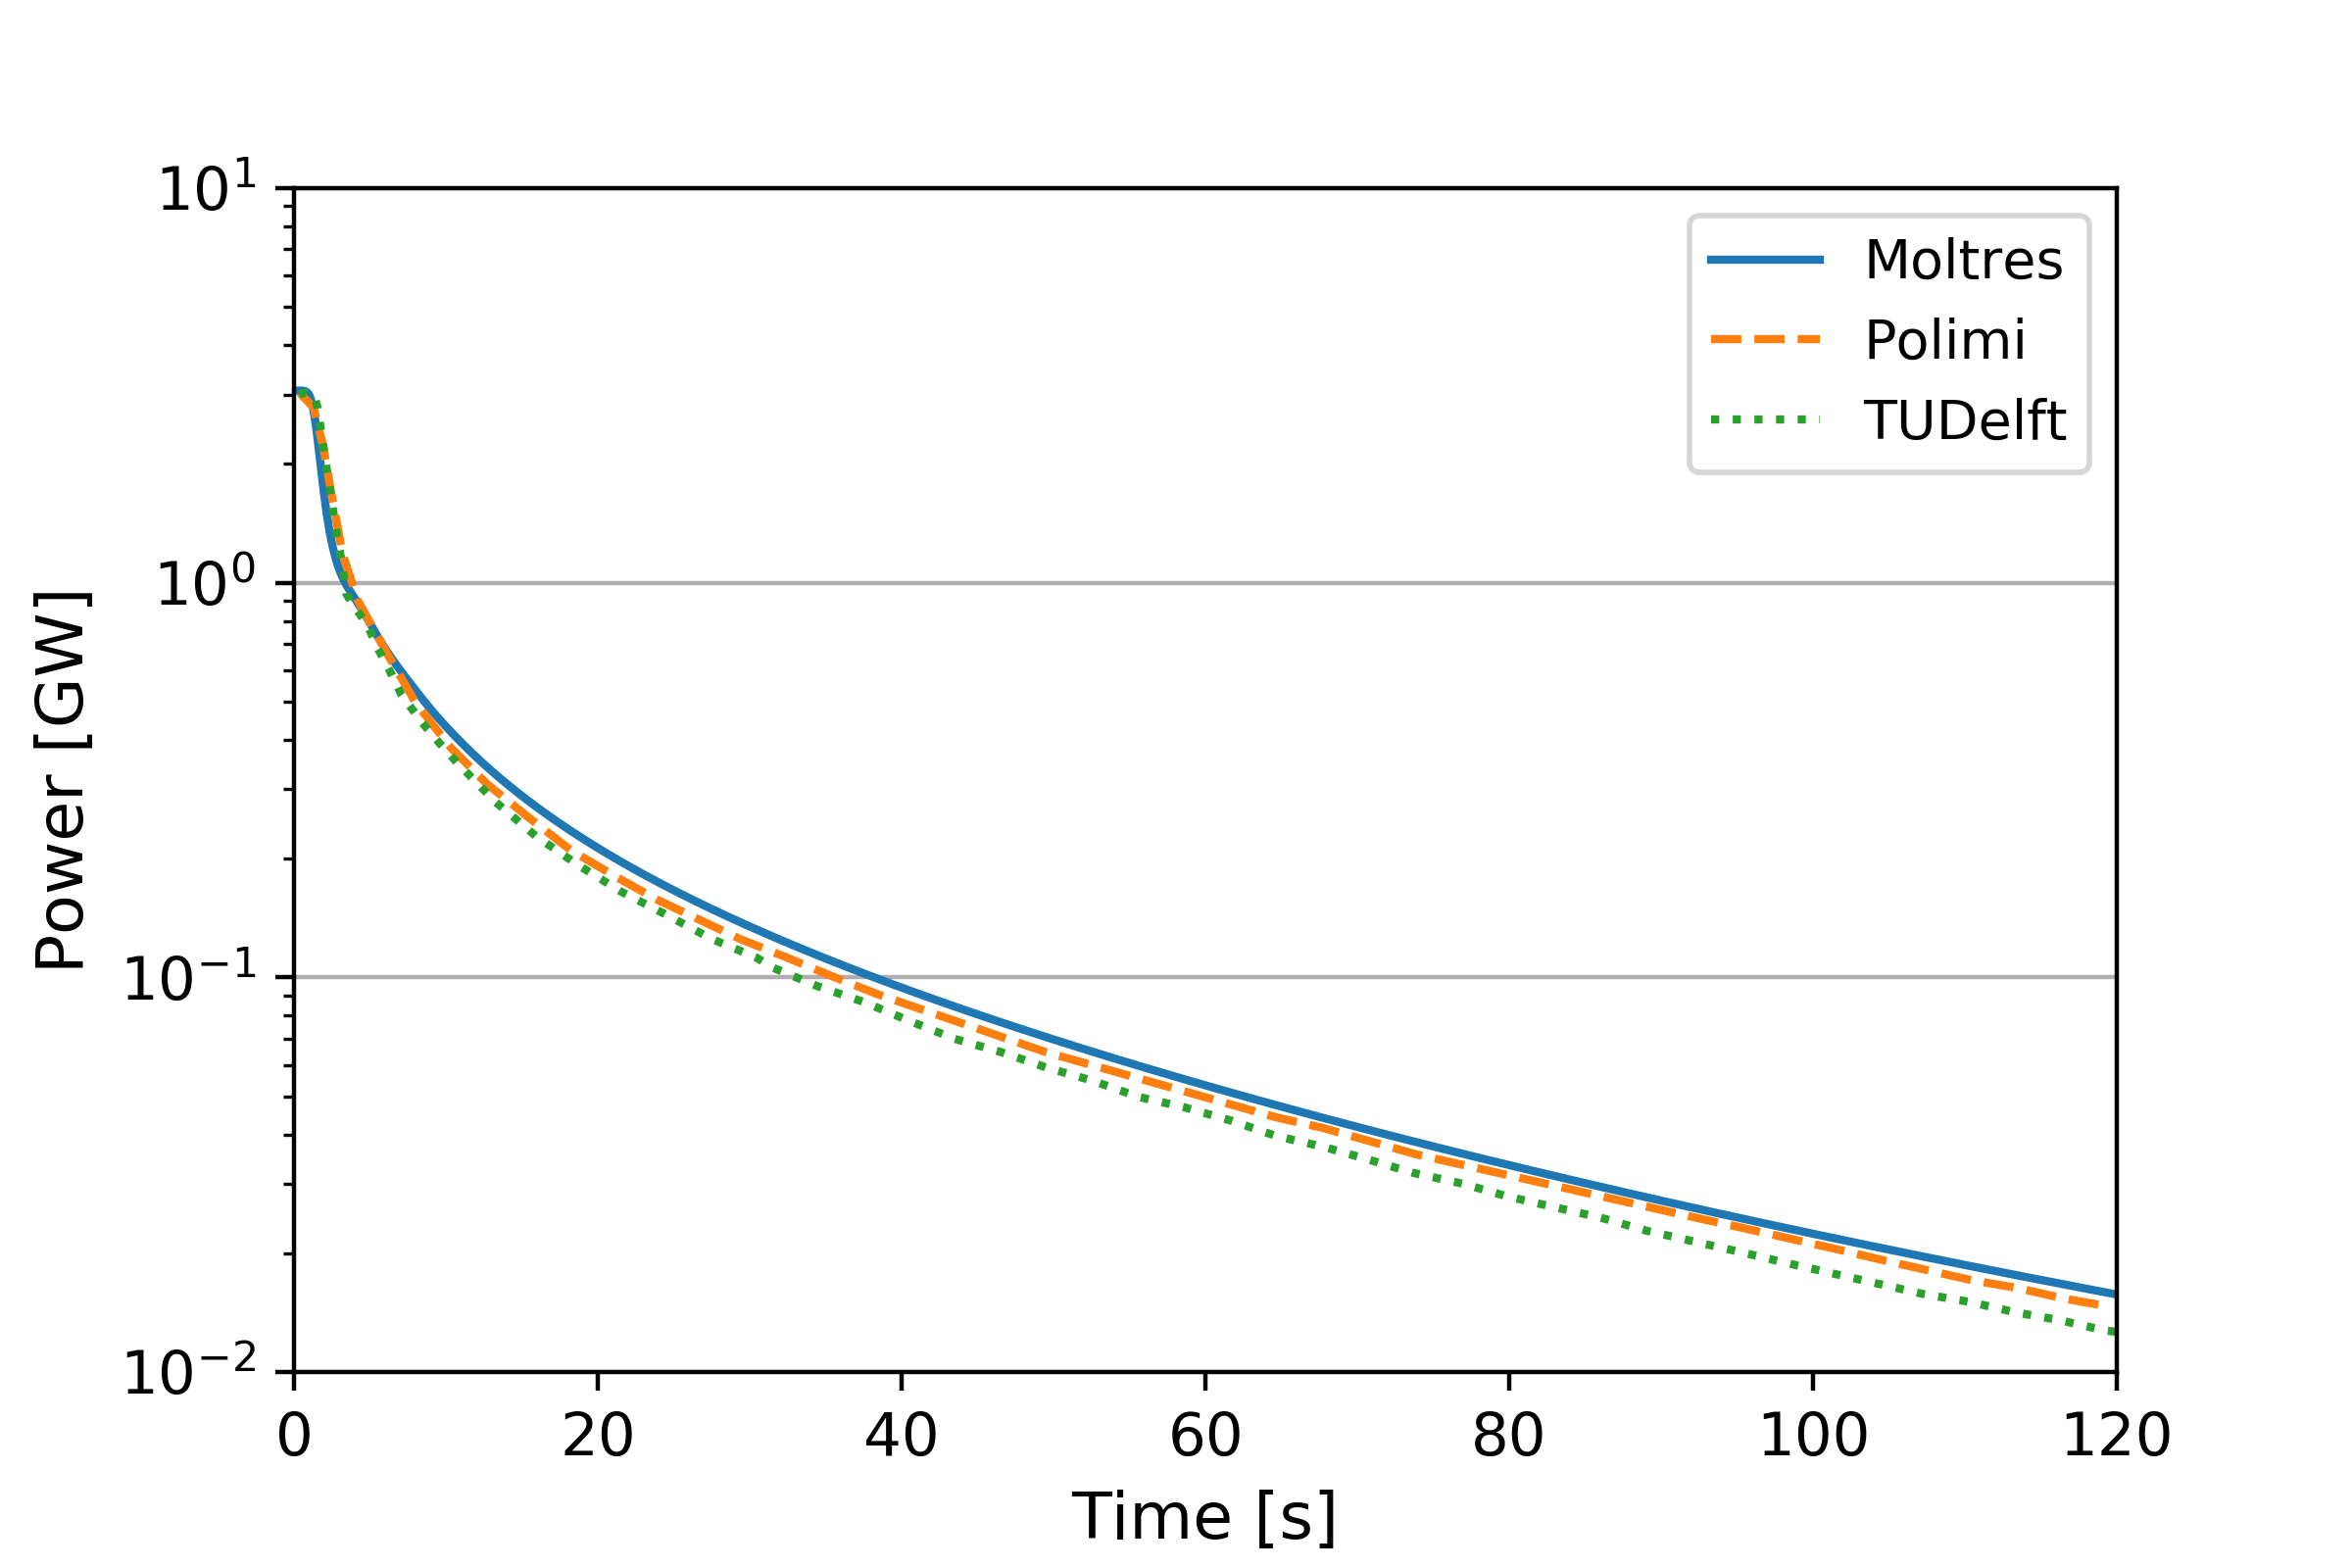
\includegraphics[width=\textwidth]{lohs-heat}
      \caption{Power output during
        an unprotected loss of heat sink transient in the Moltres, PoliMi, and
        TU Delft models \cite{fiorina_modelling_2014} without decay heat.}
      \label{fig:lohsheat}
    \end{subfigure}
\end{figure}

The loss of heat sink transients were performed with and without the decay heat
model as the TU Delft model did not possess this capability. As shown in
Figure \ref{fig:lohsheat}, without decay heat, all three models reported
similar power output responses following loss of cooling through the heat
exchanger modeled as an exponential decrease in heat removal rate with a time
constant of 1 s. As prompt heat generation decreases due to rising core
temperatures and the negative temperature reactivity feedback, decay heat
becomes a significant heat source. We observe this in Figure
\ref{fig:moltresdecaypower} which shows decay heat output overtaking prompt
heat output 34 s into the accident scenario. With the decay heat model, the
Moltres model shows good agreement with the PoliMi model. The temperature
increase averaged over the whole fuel salt loop falls within 10\% of the PoliMi
model (Figure \ref{fig:polimidecaytemp}).

\begin{figure}[htb!]
	\centering
	\begin{minipage}[t]{0.485\columnwidth}
	    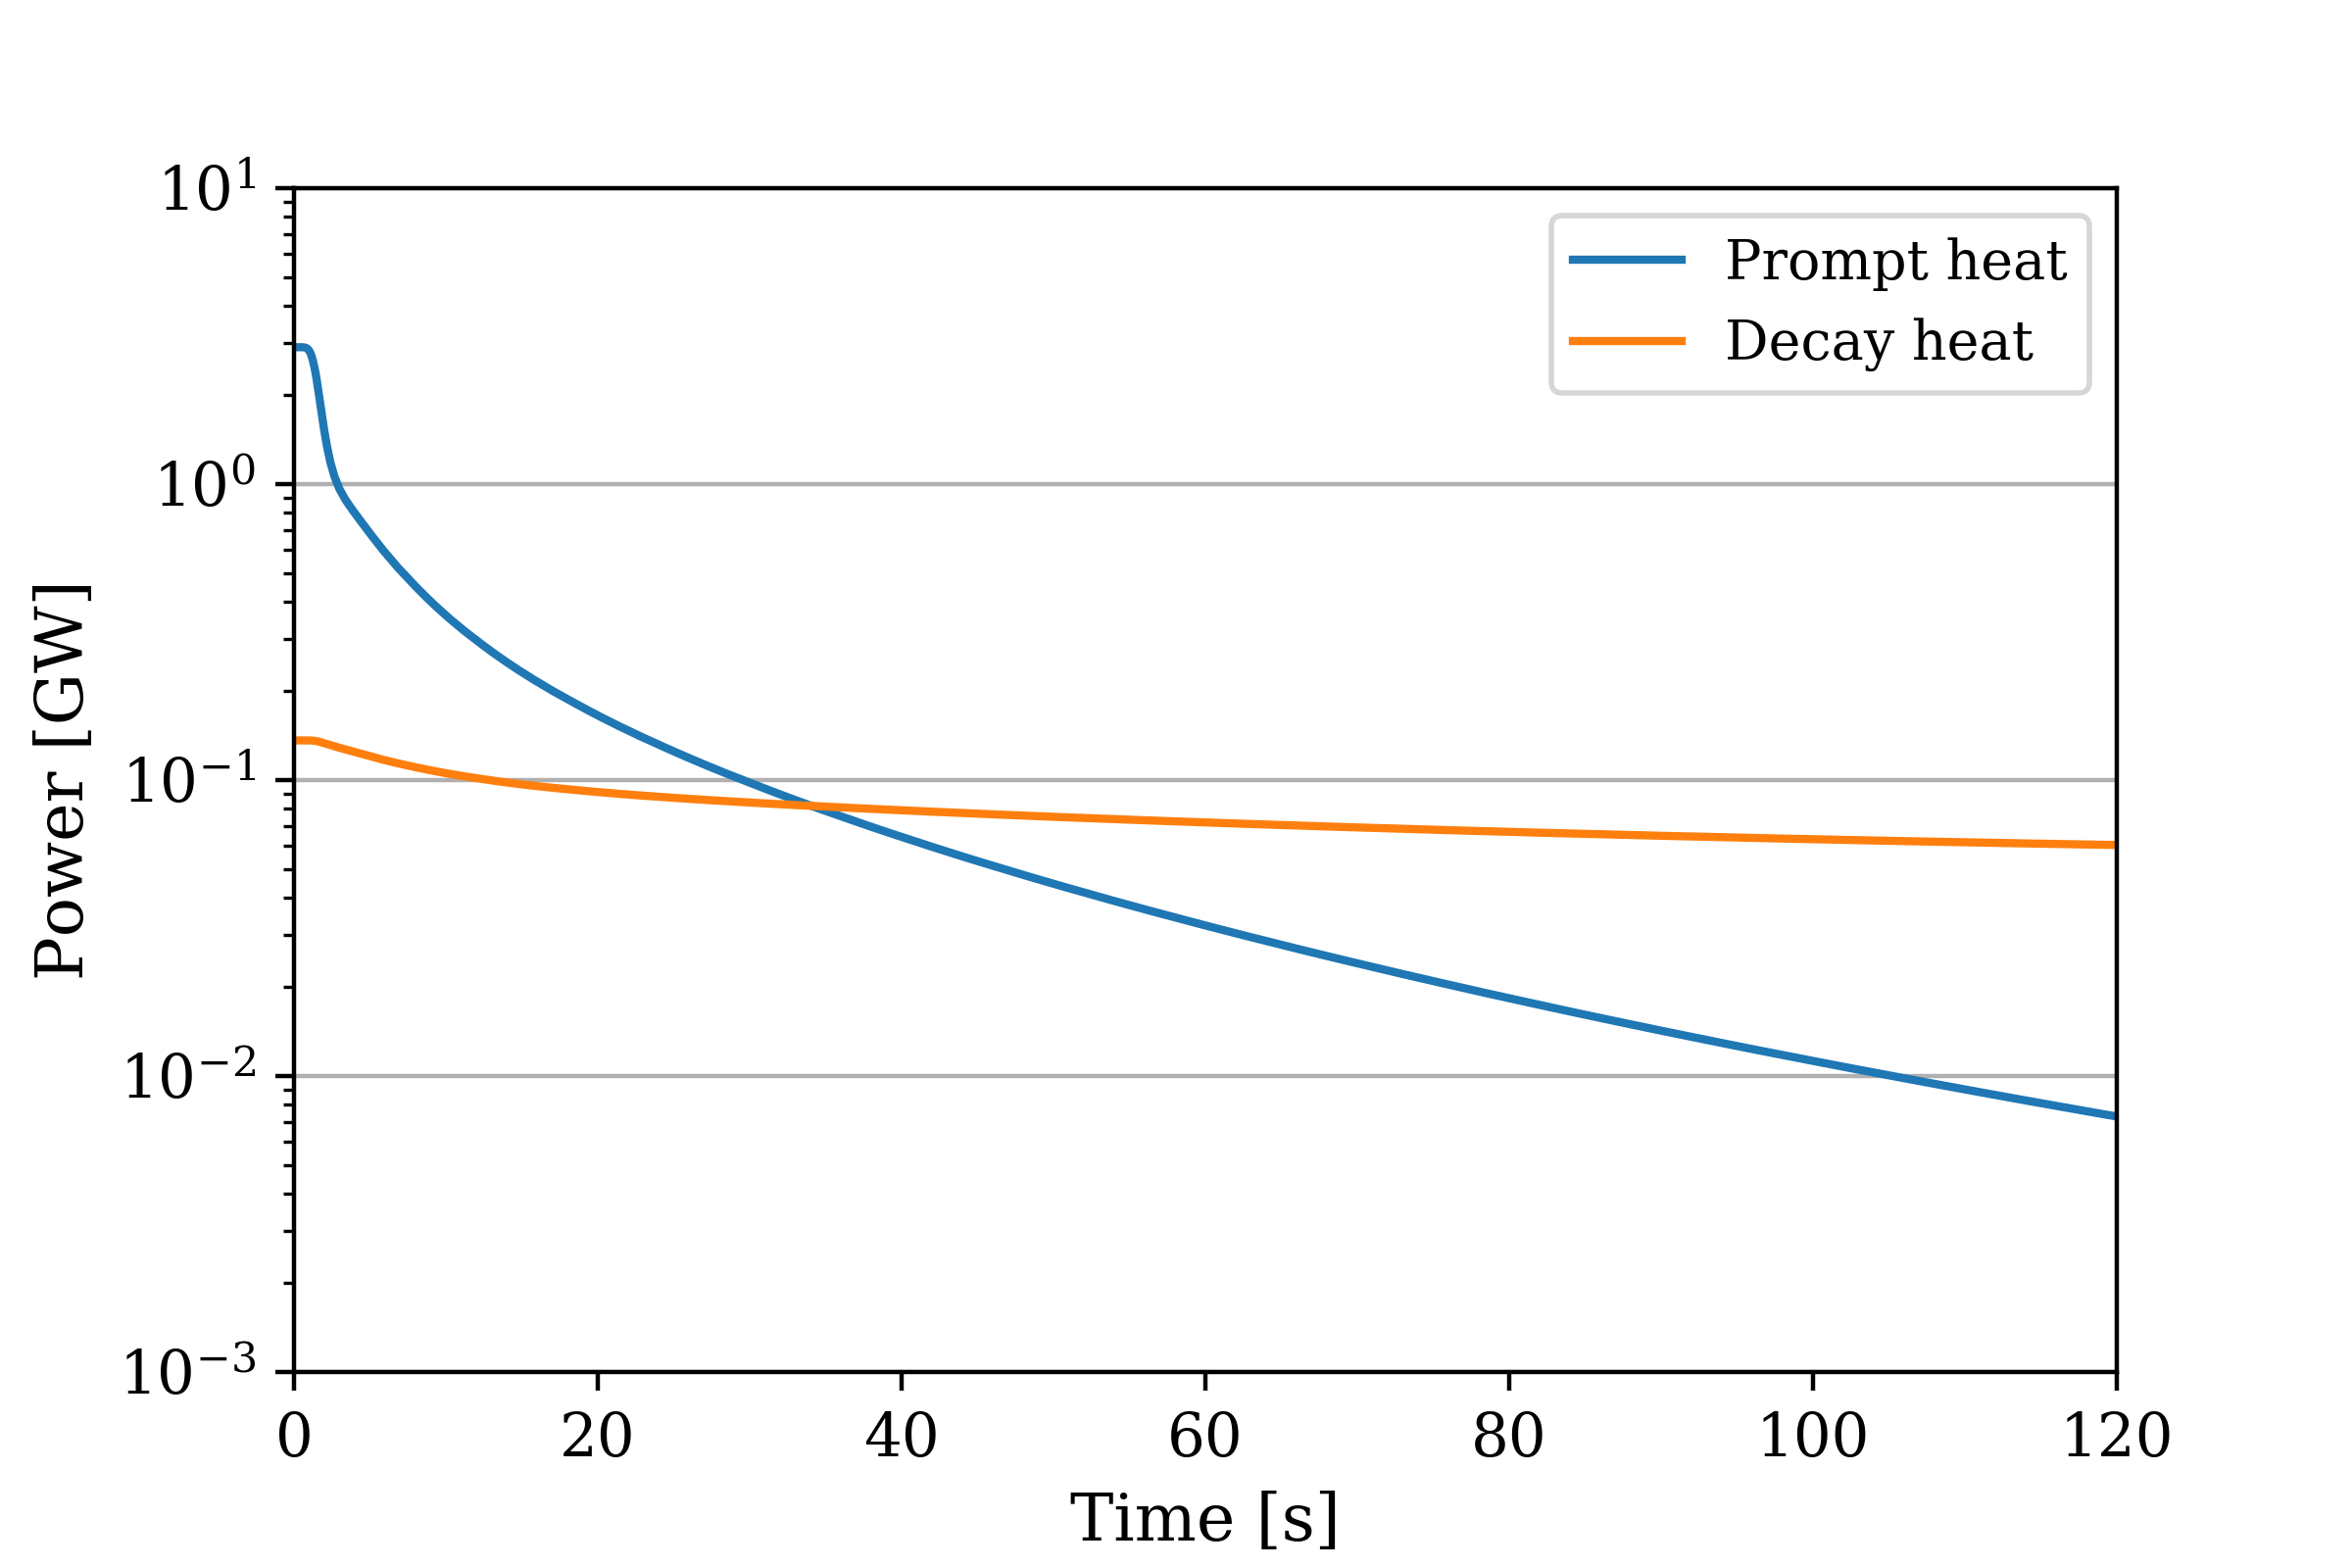
\includegraphics[width=\columnwidth]{moltres-decay-power}
	    \caption{Power output during
    an unprotected loss of heat sink transient in the Moltres model with
    decay heat.}
	    \label{fig:moltresdecaypower}
	\end{minipage}
	\hfill
	\begin{minipage}[t]{0.485\columnwidth}
	    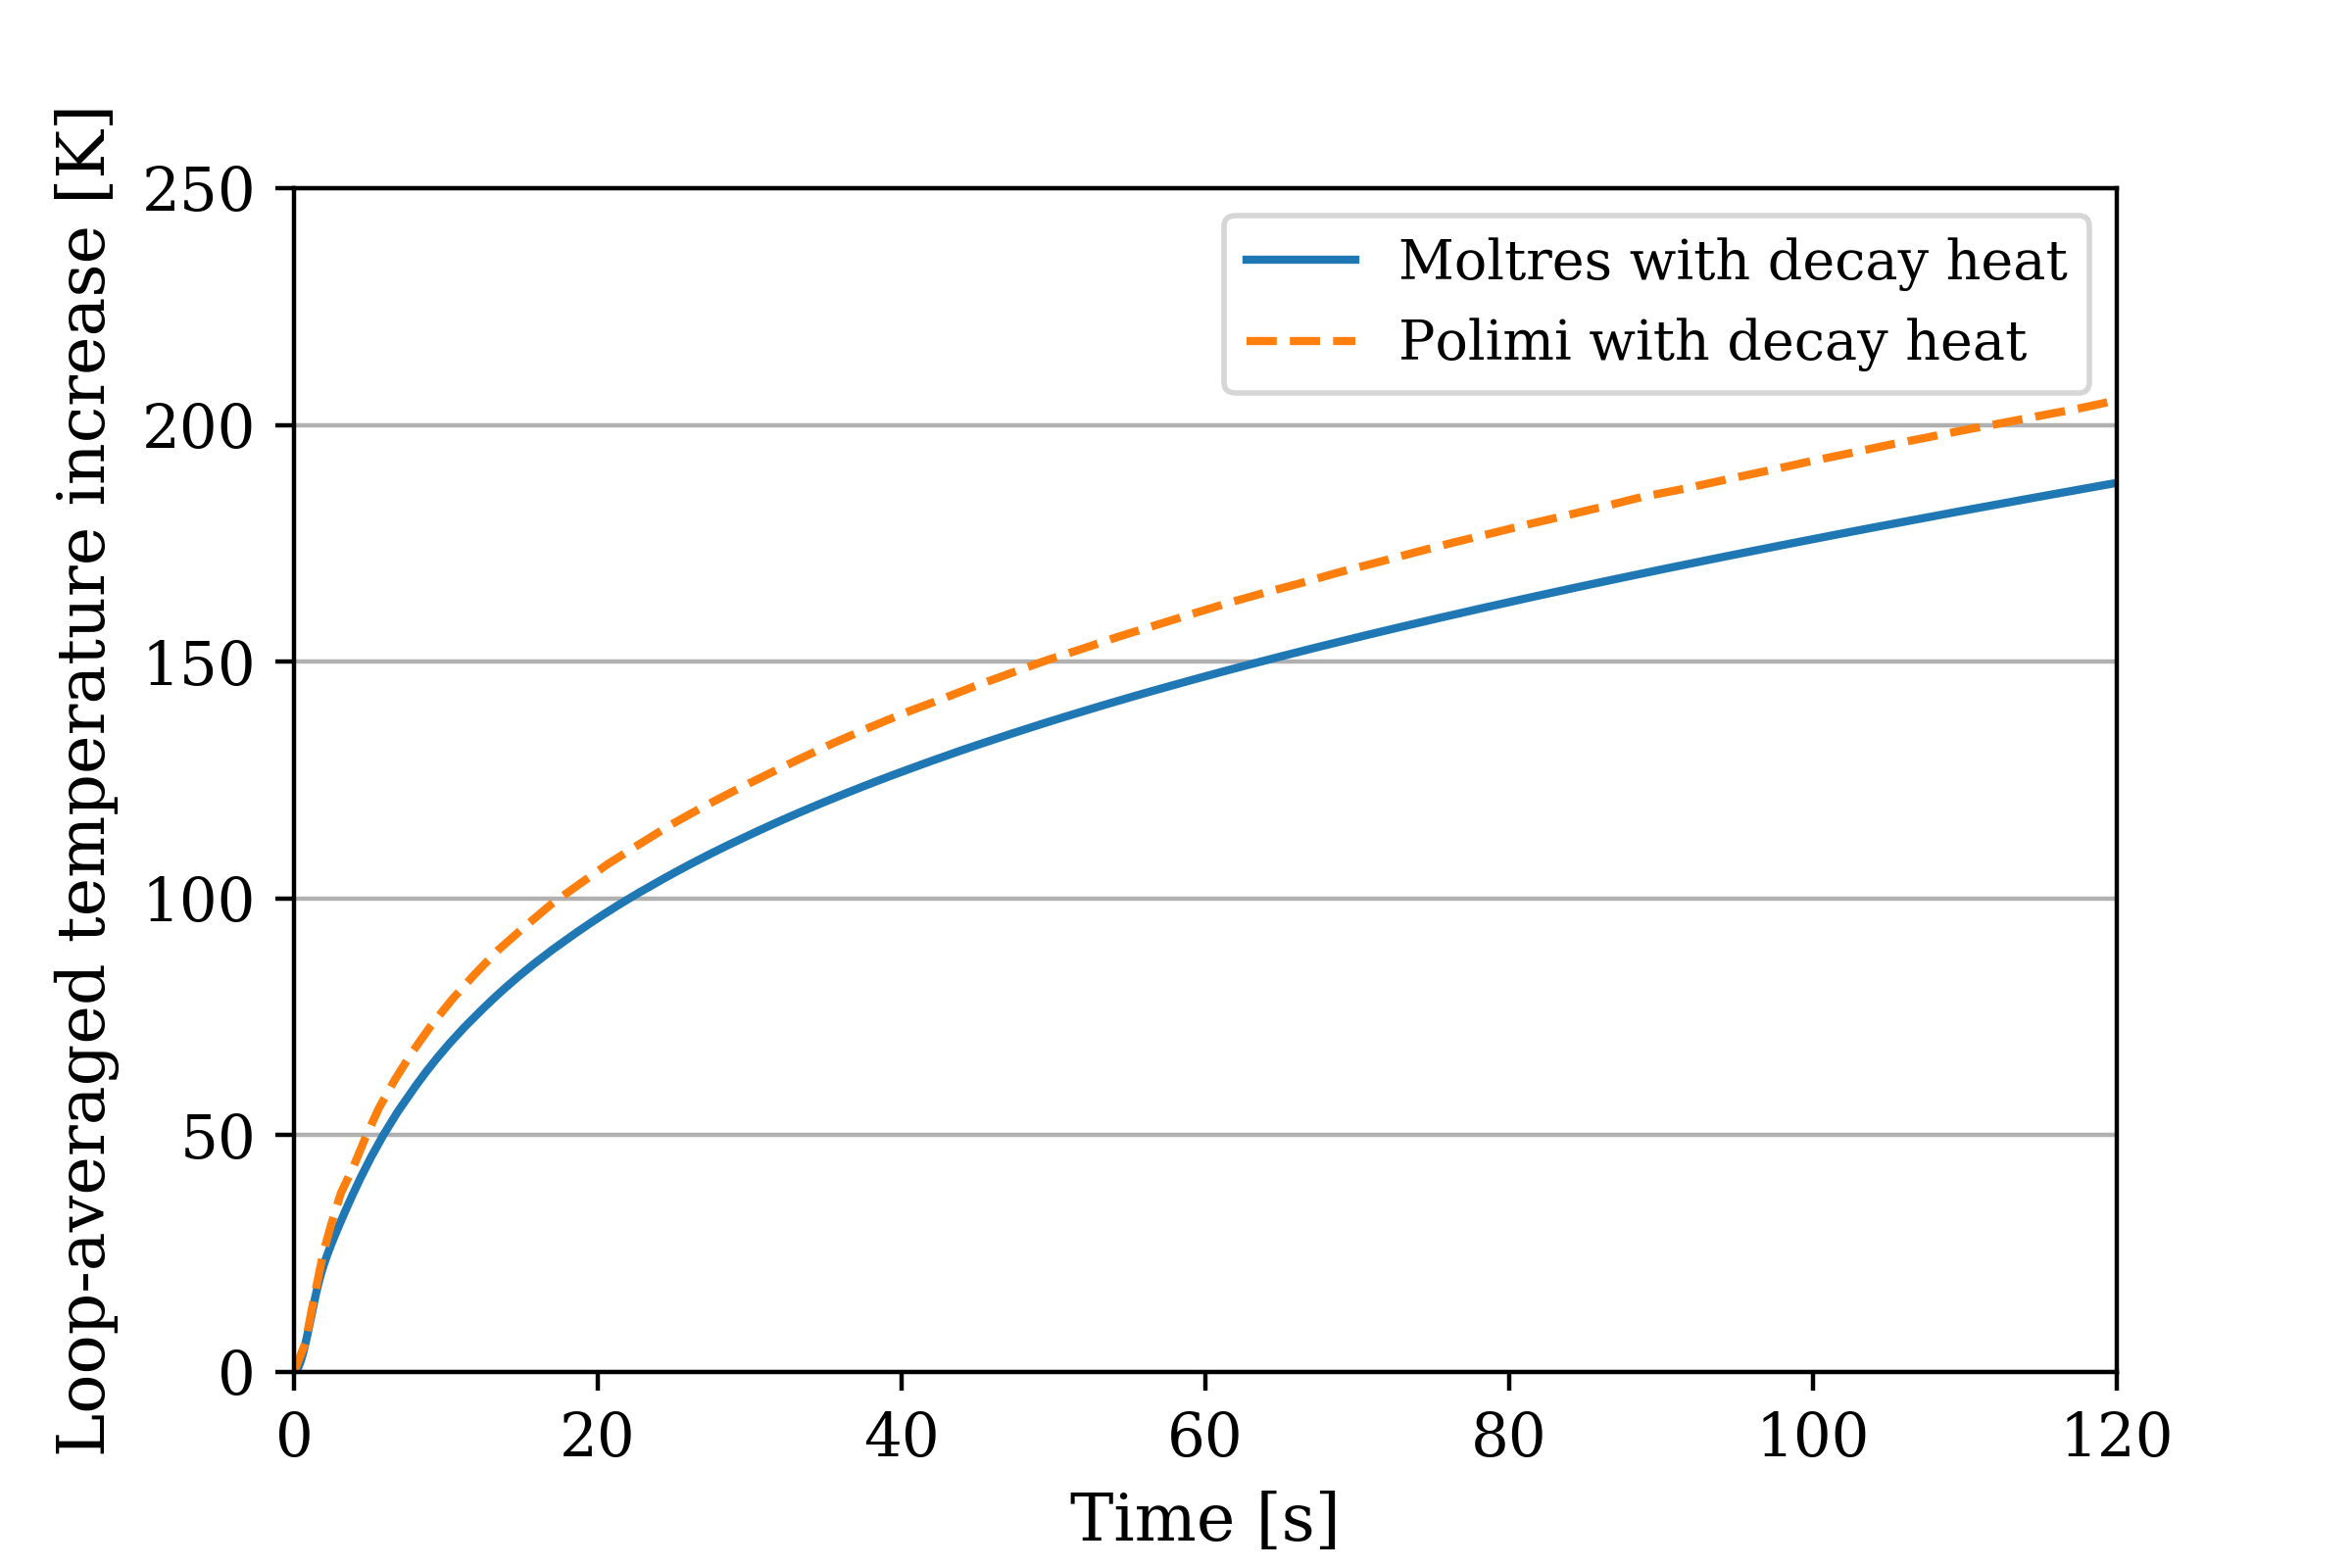
\includegraphics[width=\columnwidth]{decay-temp}
	    \caption{Loop-averaged temperature increase during
    an unprotected loss of heat sink transient in the Moltres and PoliMi
    models \cite{fiorina_modelling_2014} with decay heat.}
	    \label{fig:polimidecaytemp}
	\end{minipage}
\end{figure}

On the other hand, for the pump-initiated accident scenarios, significant
changes in the flow affected the validity of the uniform turbulent viscosity
assumption. These transients required ad hoc adjustments to the uniform
turbulent viscosity assumption as a function of volumetric flow to reproduce
the trends observed in the PoliMi and TU Delft models. Furthermore, unlike the
other two models, the Moltres model did not apply the Boussinesq approximation
for buoyancy-driven flow. The Moltres model could replicate expected trends in
the pump overspeed scenario (Figure \ref{fig:poshort}), but performed
poorly in the loss of flow scenario (Figure \ref{fig:lof}). In the latter
scenario, buoyancy effects become significant as the model loses forced flow.

\begin{figure}[htb!]
    \centering
    \begin{subfigure}[t]{.485\textwidth}
        \centering
        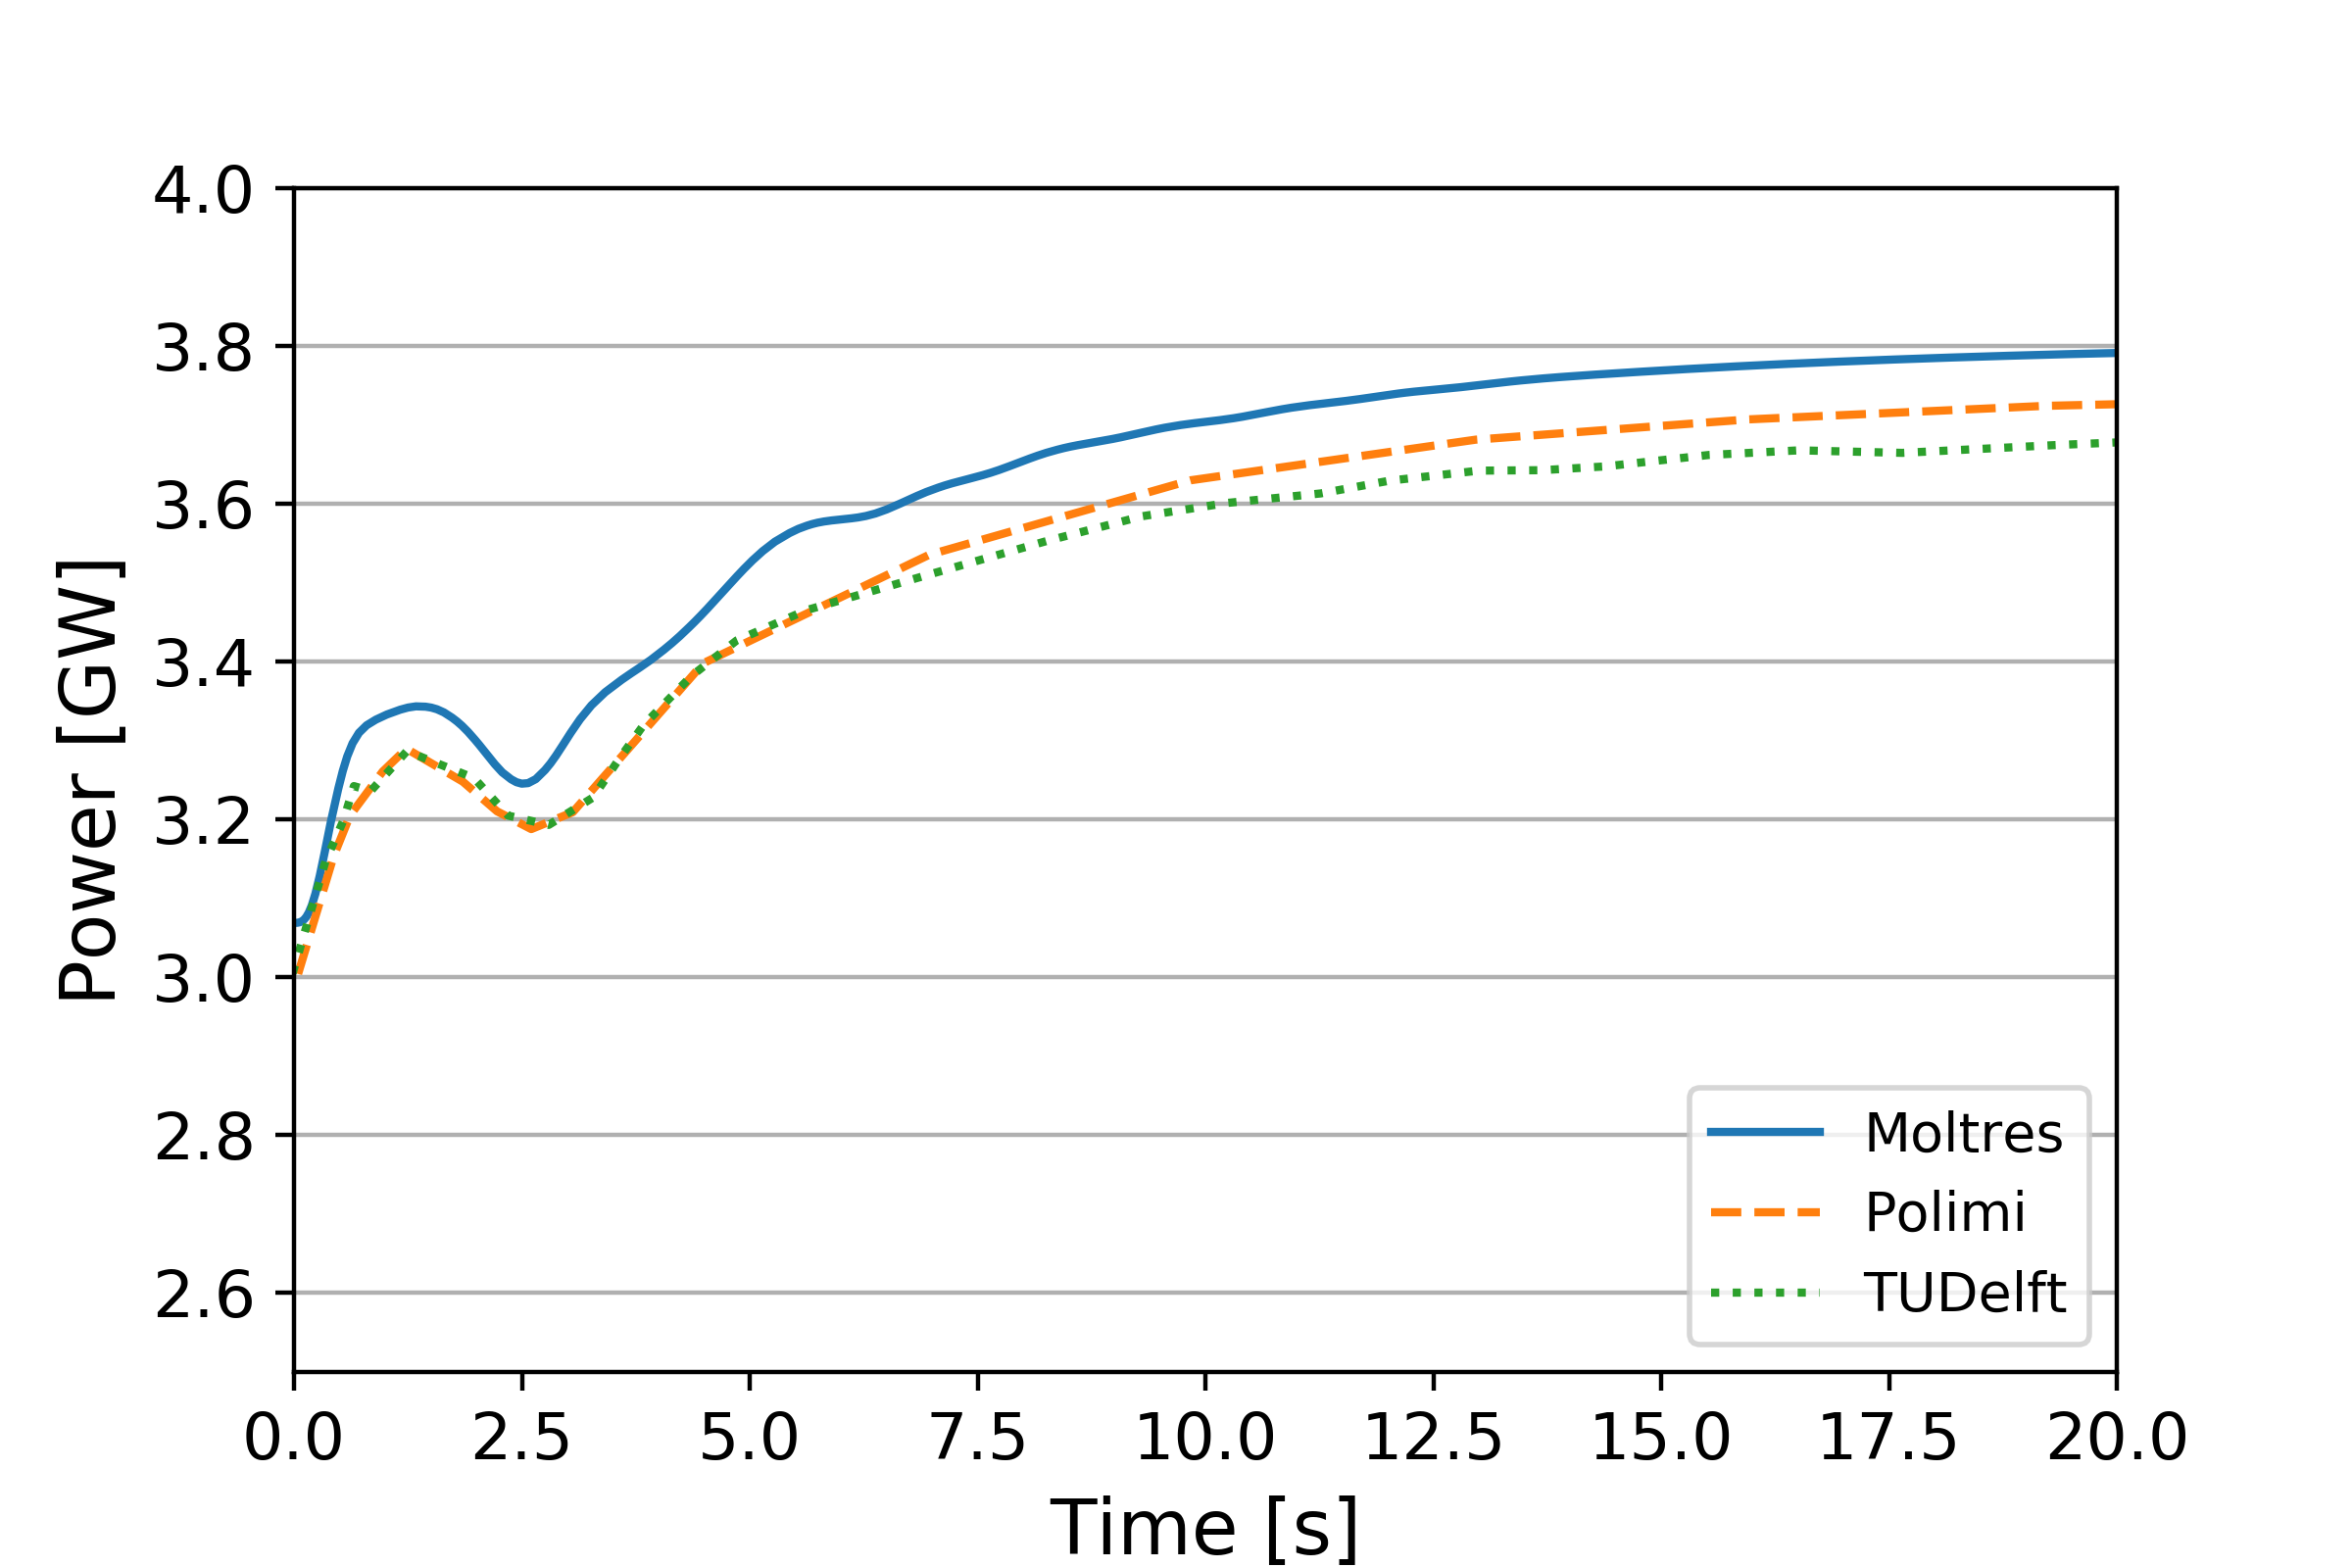
\includegraphics[width=\textwidth]{po-heat-short}
    \end{subfigure}
    \hfill
    \begin{subfigure}[t]{.485\textwidth}
        \centering
        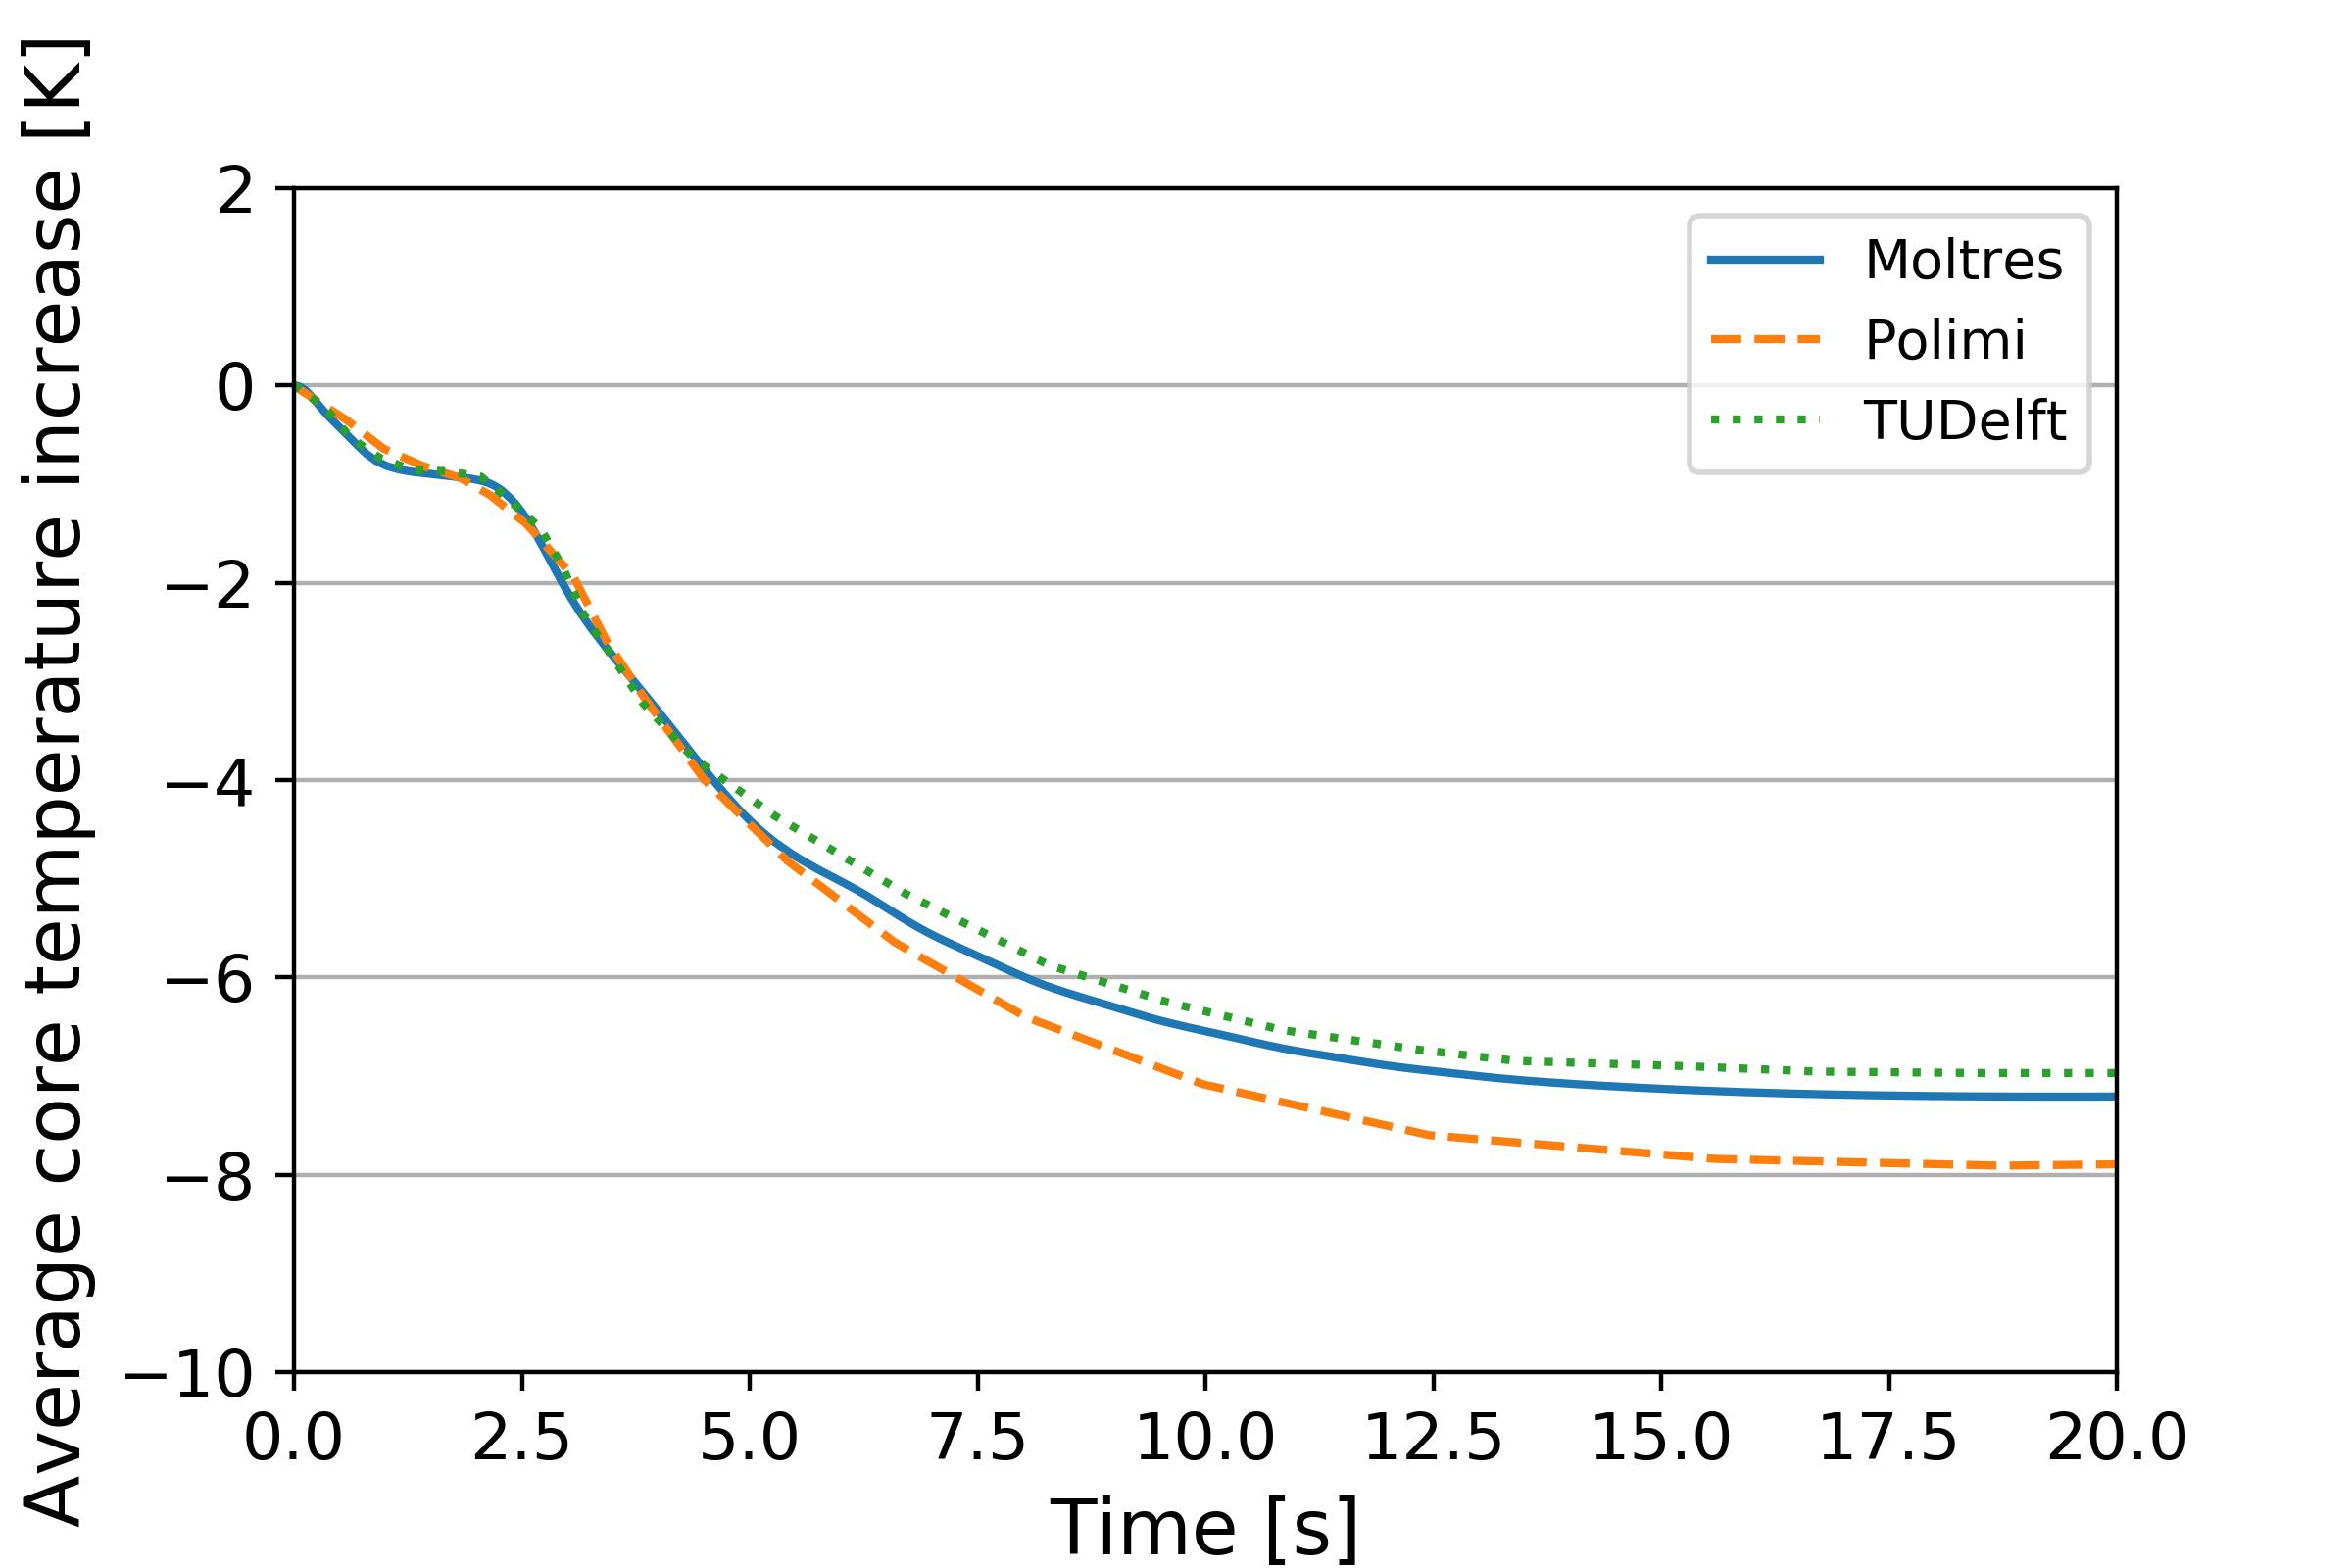
\includegraphics[width=\textwidth]{po-temp-short}
    \end{subfigure}
    \caption{Average core temperature increase during
    an unprotected pump overspeed transient in the Moltres, PoliMi, and
    TU Delft models \cite{fiorina_modelling_2014}.}
    \label{fig:poshort}
\end{figure}

\begin{figure}[htb!]
    \centering
    \begin{subfigure}[t]{.485\textwidth}
        \centering
        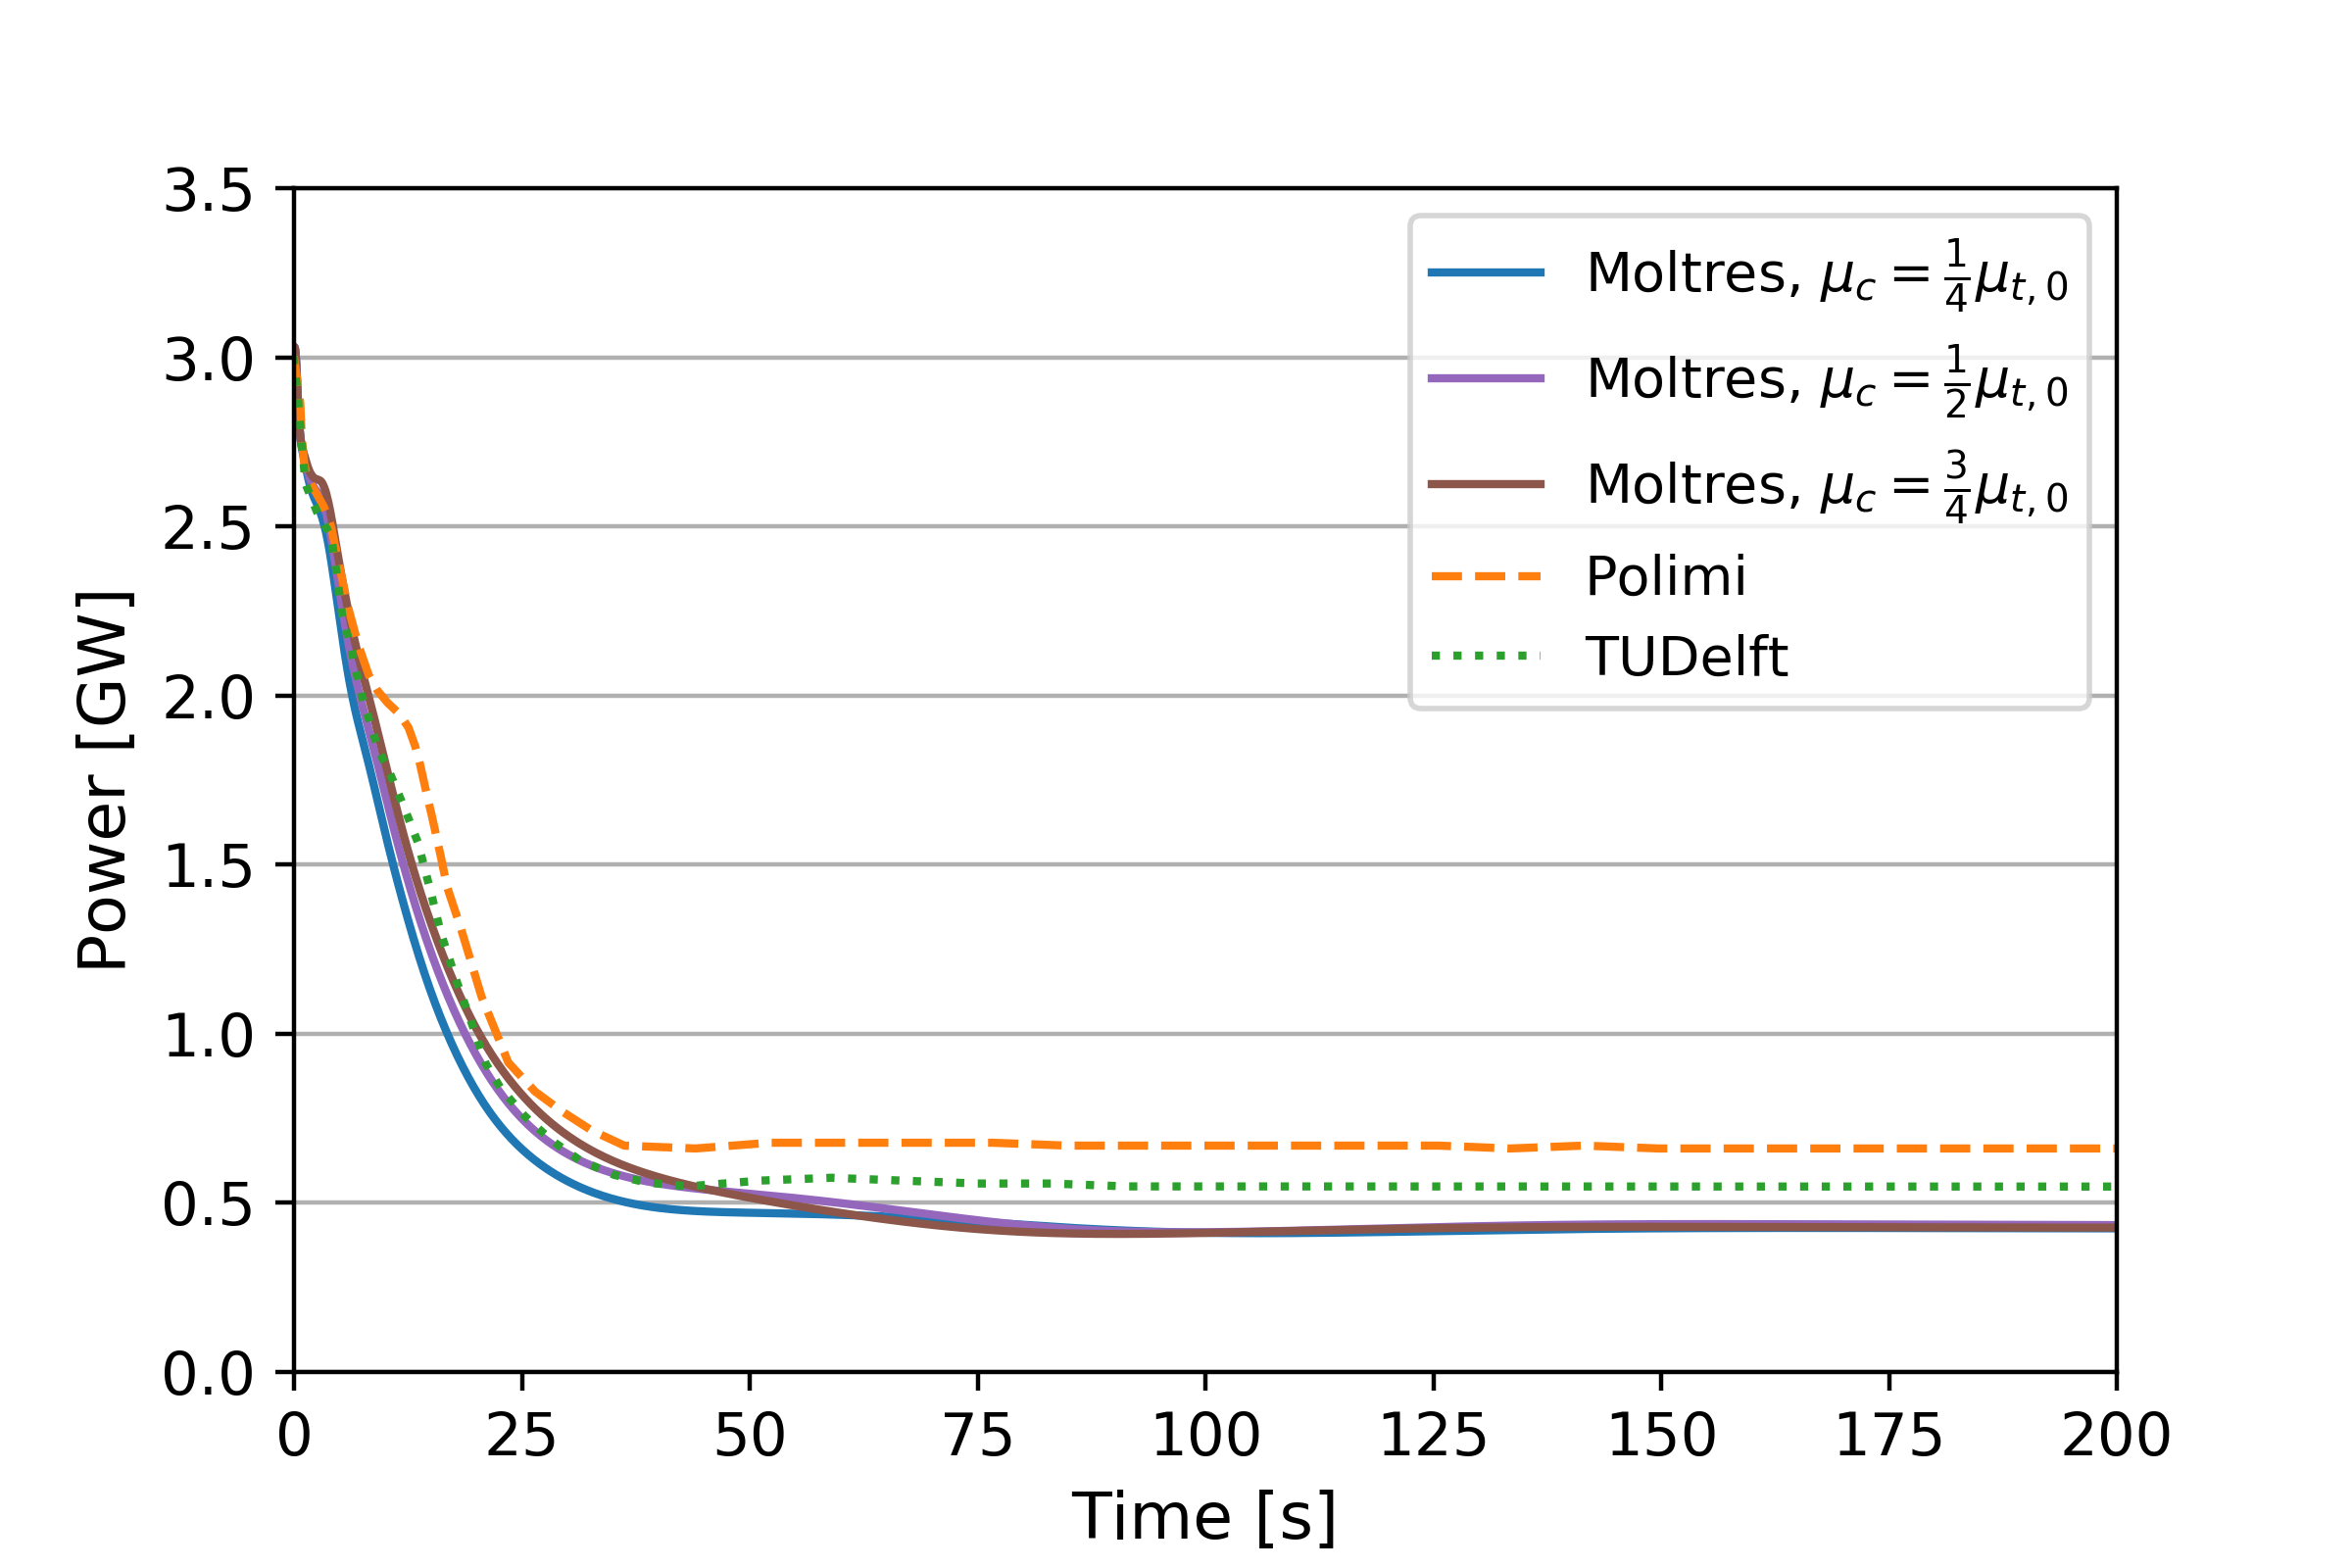
\includegraphics[width=\textwidth]{lof-heat}
    \end{subfigure}
    \hfill
    \begin{subfigure}[t]{.485\textwidth}
        \centering
        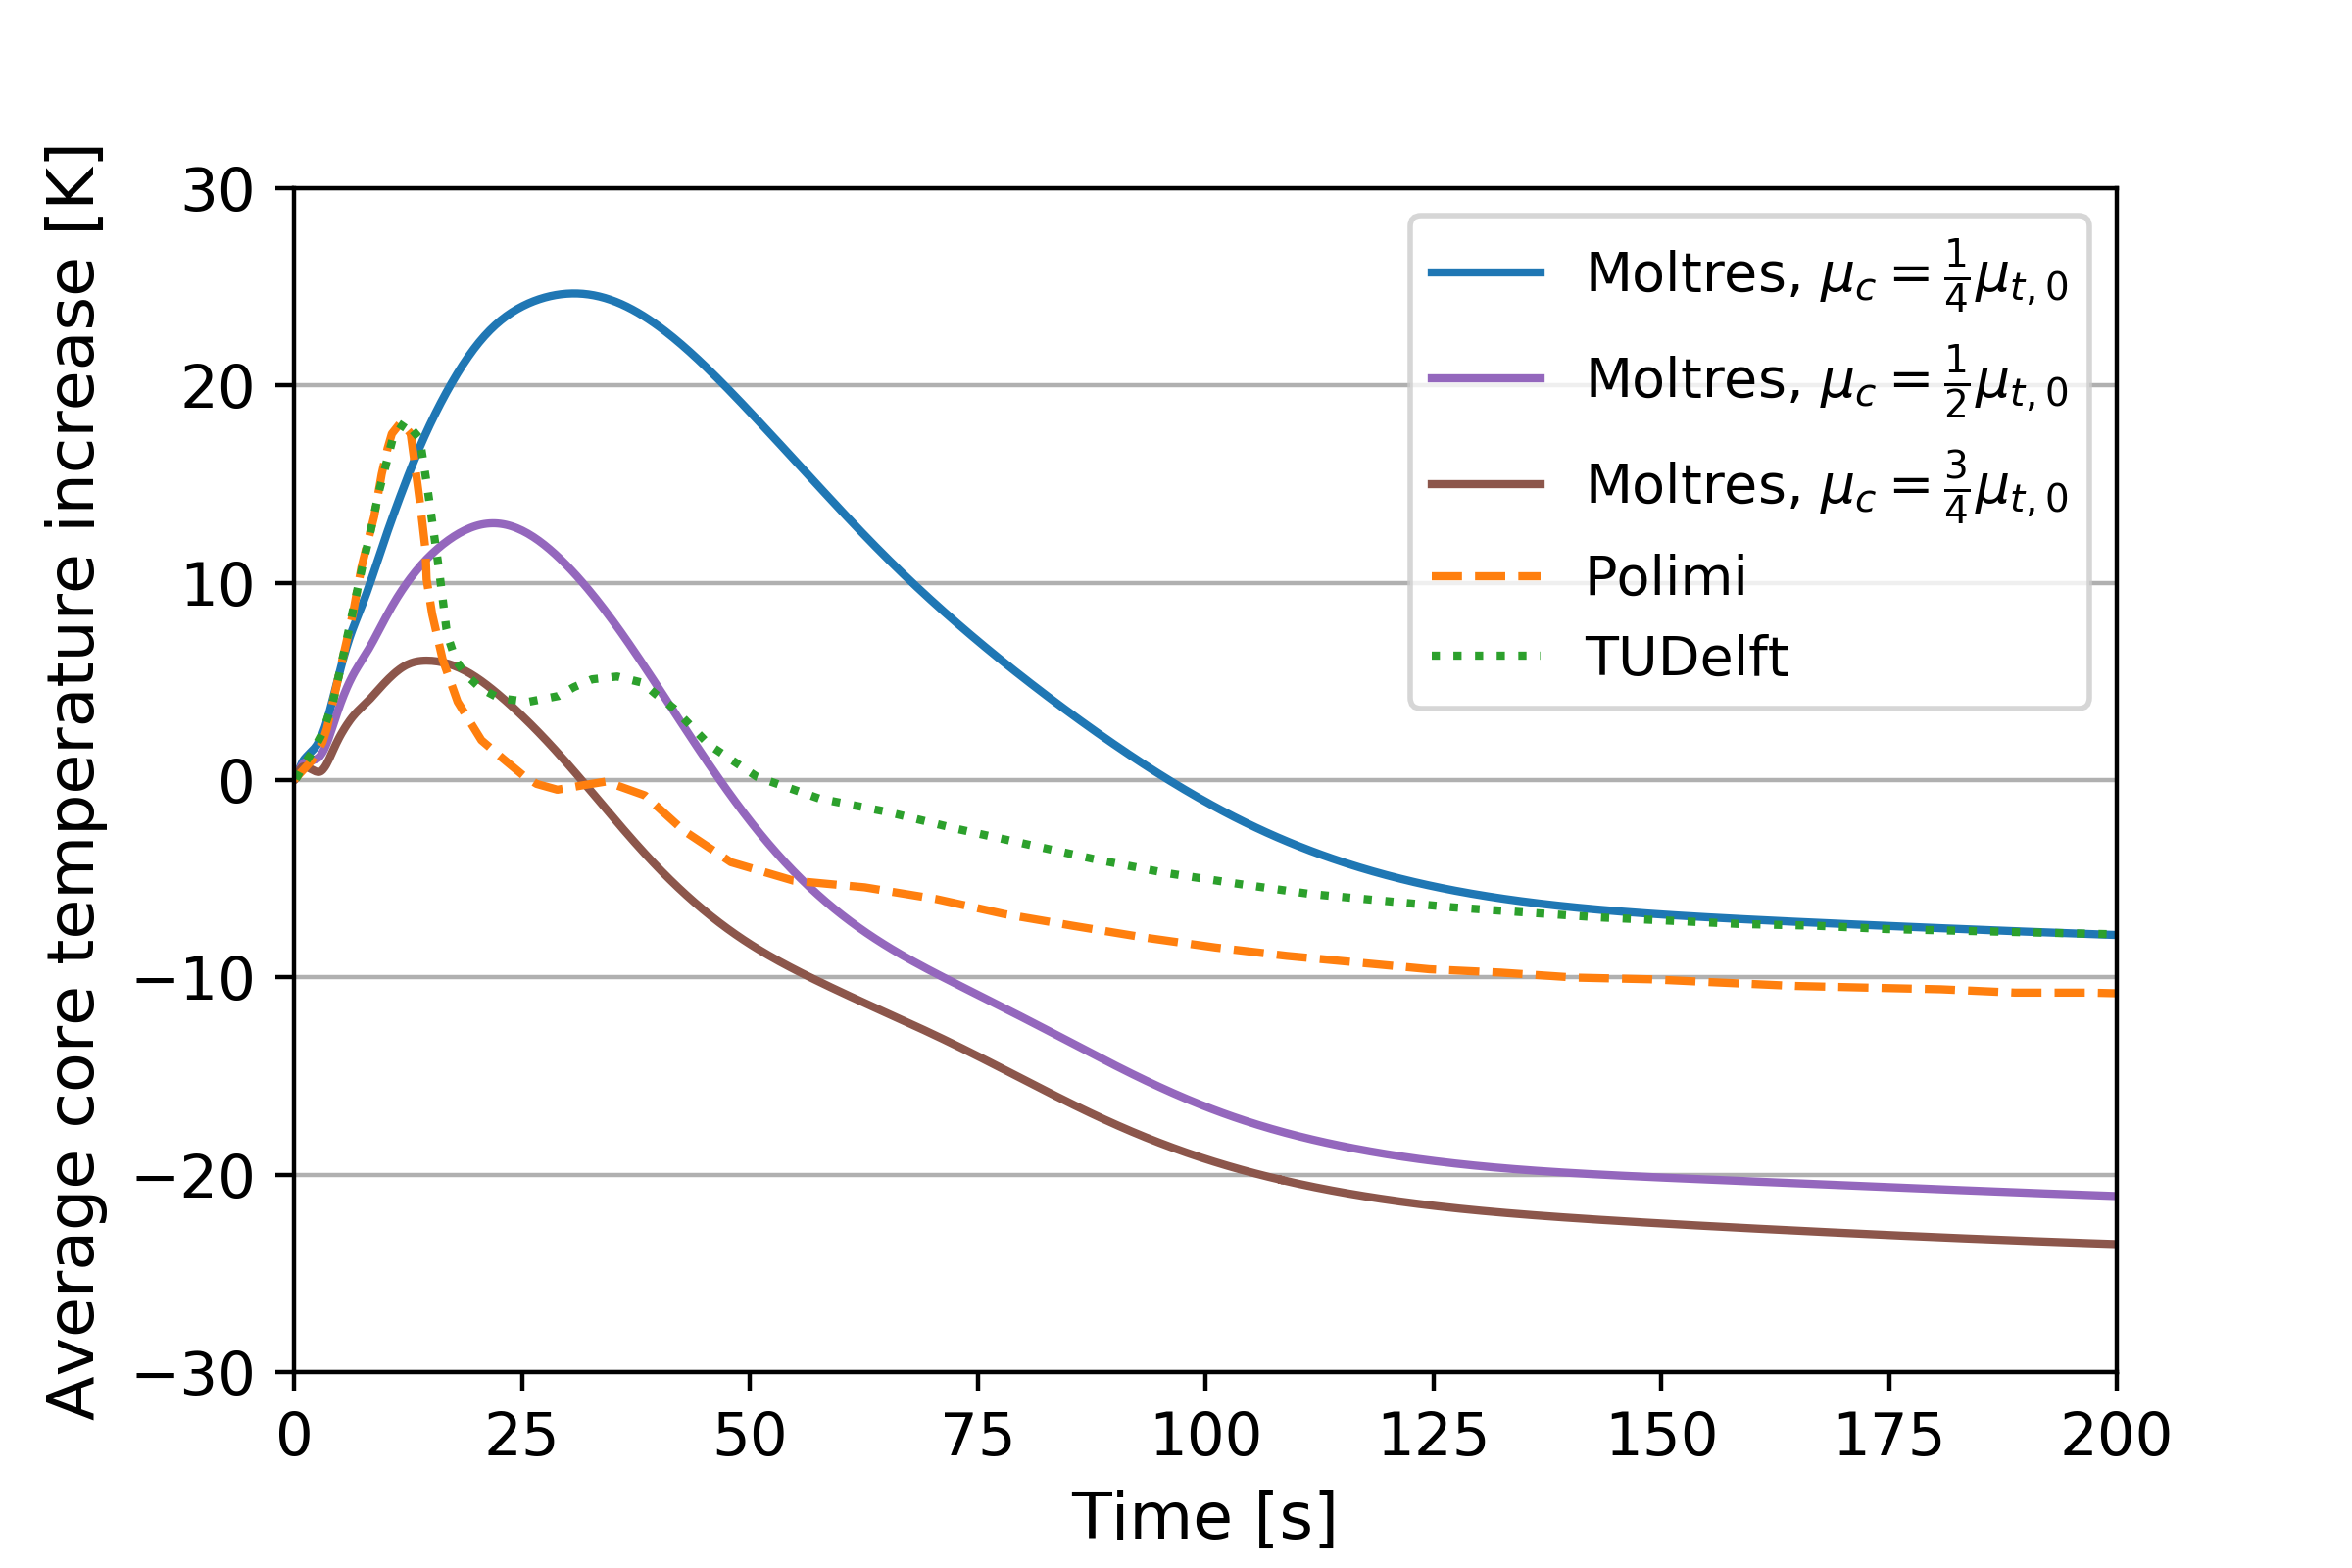
\includegraphics[width=\textwidth]{lof-temp}
    \end{subfigure}
    \caption{Power output and average core temperature increase during
    an unprotected loss of flow transient in the Moltres, PoliMi, and
    TU Delft models \cite{fiorina_modelling_2014}.}
    \label{fig:lof}
\end{figure}

\subsubsection{Critical Assessment} \label{sec:msfr-critique}

Given the inherent and unique characteristics of \glspl{MSR}, the new
capabilities introduced in this work---coupling to incompressible Navier-Stokes
equations, precursor loop system, and decay heat model---are essential for
accurate \gls{MSR} modeling and simulation. This work demonstrated these
capabilities through steady-state and transient studies of a 2D axisymmetric
\gls{MSFR} model similar to models by Fiorina et al.
\cite{fiorina_modelling_2014} and Aufiero et al.
\cite{aufiero_development_2014}. The Moltres model showed good agreement with
the other models in
most steady-state and transient cases with respect to the neutron flux, reactor
power, temperature, and velocity distributions. Most crucially, the
incompressible flow model reproduced characteristic regions of recirculating
flow and near-stagnant flow observed in the PoliMi and TU Delft \gls{MSFR}
models which led to the formation of temperature hotspots and precursor
accumulation in the core.

However, significant discrepancies observed during pump-initiated transient
scenarios highlight the need for a proper turbulence model to capture
turbulent flow effects in some \gls{MSR} designs. Unlike the \gls{MSRE}, the
\gls{MSFR} experiences highly turbulent flow whose Reynolds number is on the
order of $10^6$ under normal operating conditions. This level of turbulent flow
produces eddies of a wide range of length scales, and the computational demands
of the fine mesh and time resolution render it numerically unsolvable with
today's computational resources. Turbulence models allow for cheaper turbulence
simulations on coarser meshes by approximating the turbulent effects through
statistical analysis. Fiorina et al. \cite{fiorina_modelling_2014} employed the
$k$-$\epsilon$ turbulence model in their PoliMi and TU Delft models. Moltres
will benefit from coupling to similar intermediate-fidelity turbulence models
for turbulence simulations at reasonable computational costs.

While the Moltres model demonstrated good agreement with published data in the
steady-state, reactivity, and loss of heat sink scenarios, this work does not
provide rigorous verification of Moltres' capabilities for \gls{MSR} modeling.
The \gls{MSFR} simulations involve various physics models which combine to form
a complex multiphysics model. Therefore, it is difficult to pinpoint sources of
discrepancy with a high degree of certainty. Differences in the modeling
approaches also introduce discrepancies which cannot be reliably identified.
Moving forward, Moltres will benefit from code-to-code verification of
individual components responsible for modeling various physics present in
\glspl{MSR} as well as the multiphysics coupling approach.
